\documentclass[sigconf, balance=false]{acmart}

\setcopyright{acmlicensed}
\copyrightyear{2026}
\acmYear{2026}
\acmDOI{XXXXXXX.XXXXXXX}

\acmConference[ACM Conf '26]{Make sure to enter the correct conference title from your rights confirmation email}{2026}{Location, Country}
\acmISBN{978-1-4503-XXXX-X/2026/XX}

\AtBeginDocument{%
  \providecommand\BibTeX{{%
    Bib\TeX}}}

\usepackage{tikz}
\usetikzlibrary{shapes.geometric, arrows.meta, positioning, fit, backgrounds, calc}
\usepackage{booktabs}
\usepackage{tabularx}
\usepackage{array}
\usepackage{multirow}
\usepackage{stfloats}
\usepackage{placeins}
\usepackage{enumitem}
\usepackage{xurl}
\usepackage{amsmath}
% Undefine \Bbbk if already defined by newtxmath (acmart) to prevent conflict with amssymb
\let\Bbbk\relax
\usepackage{amssymb}

% Custom colors for TikZ and annotations
\definecolor{amber}{rgb}{1.0, 0.75, 0.0}

% Relax line-breaking penalties in narrow two-column layout to prevent margin overflows
\emergencystretch=1.5em
\sloppy

% Tune float placement parameters so figures and tables stay close to their text
\renewcommand{\topfraction}{0.95}
\renewcommand{\bottomfraction}{0.95}
\renewcommand{\textfraction}{0.05}
\renewcommand{\floatpagefraction}{0.85}
\renewcommand{\dbltopfraction}{0.95}
\renewcommand{\dblfloatpagefraction}{0.85}
\setcounter{topnumber}{5}
\setcounter{bottomnumber}{5}
\setcounter{totalnumber}{10}
\setcounter{dbltopnumber}{5}

\begin{document}

\title[The Cloud-Native Observability Maturity Model (CN-OMM)]{The Cloud-Native Observability Maturity Model (CN-OMM): A Design Science Formalization, Automated Assessment Protocol, and Empirical Chaos Validation}

\author{Fagner Silva}
\authornote{Both authors contributed equally to this research.}
\affiliation{%
  \institution{Centro de Inform\'{a}tica, UFPE}
  \city{Recife}
  \state{Pernambuco}
  \country{Brazil}
}
\email{ffcs@cin.ufpe.br}
\orcid{0000-0000-0000-0000}

\author{Jackson Raniel}
\affiliation{%
  \institution{Universidade de Pernambuco - Campus Caruaru}
  \city{Caruaru}
  \state{Pernambuco}
  \country{Brazil}
}
\email{jackson.florencio@upe.br}

\author{Vin\'{i}cius Cardoso Garcia}
\authornotemark[1]
\affiliation{%
  \institution{Centro de Inform\'{a}tica, UFPE}
  \city{Recife}
  \state{Pernambuco}
  \country{Brazil}
}
\email{vcg@cin.ufpe.br}

\renewcommand{\shortauthors}{Silva et al.}

\begin{abstract}
Modern cloud-native microservices orchestrated by Kubernetes exhibit high topological dynamism and stochastic failure modes that render traditional reactive monitoring insufficient. To guide architectural evolution, industry vendors and recent preliminary studies have proposed observability maturity frameworks. However, a systematic inspection reveals that existing proposals suffer from three structural flaws: (i) \textit{vendor lock-in bias} that conflates maturity with telemetry volume rather than causal diagnostic capability; (ii) \textit{probe effect blindness} that ignores the CPU and memory overhead imposed by deep instrumentation; and (iii) the \textit{monomodal additivity fallacy}, which assumes that adopting isolated telemetry pillars (e.g., distributed tracing) monotonically improves fault localization. Furthermore, over $50\%$ of maturity models in software engineering lack empirical validation (the ``Validation Gap''). Grounded in Design Science Research (DSR) guidelines (Hevner et al.; Becker et al.; De Bruin et al.), Process Theory, and Configurational Equifinality, this paper formalizes the \textbf{Cloud-Native Observability Maturity Model (CN-OMM)}. Structurally, CN-OMM defines a $5\text{-Level} \times 5\text{-Dimension}$ stage-gate matrix spanning 15 capability sub-components: (D1) Telemetry Acquisition \& Depth, (D2) Semantic Context \& Cross-Pillar Correlation, (D3) Diagnostic \& Analytical Intelligence, (D4) Resilience Verification \& SLO Governance, and (D5) Instrumentation Economics \& Probe Effect Governance. To replace subjective Likert questionnaires, we introduce an \textbf{Automated Maturity Assessment Protocol} featuring 15 Quantitative Capability Indicators (QCIs) and a non-compensatory mathematical scoring function. Finally, we conduct a Type-3 real-system empirical validation across $N=30$ paired Chaos Engineering trials on a polyglot Kubernetes benchmark. Results demonstrate that advancing to Level 3 (monomodal tracing) without fulfilling the configurational stage-gate of semantic correlation (D2) collapses diagnostic accuracy to $0.00\%$ due to \textit{Cascading Span Bias}, whereas progressing to Level 4 (multimodal semantic correlation with exclusive self-time decomposition) elevates diagnostic accuracy to $83.33\%$ ($p = 7.74 \times 10^{-7}$) and reduces median diagnostic latency by $94.24\%$ ($300.00\,\text{s} \rightarrow 17.27\,\text{s}$, $p = 3.06 \times 10^{-5}$) while bounding steady-state CPU overhead at $9.51\% \pm 2.14\%$ ($p = 6.52 \times 10^{-9}$).
\end{abstract}

\begin{CCSXML}
<ccs2012>
   <concept>
       <concept_id>10011007.10011074.10011075</concept_id>
       <concept_desc>Software and its engineering~Software architectures</concept_desc>
       <concept_significance>500</concept_significance>
   </concept>
   <concept>
       <concept_id>10011007.10011074.10011099.10011102.10011103</concept_id>
       <concept_desc>Software and its engineering~Software testing and debugging</concept_desc>
       <concept_significance>500</concept_significance>
   </concept>
   <concept>
       <concept_id>10010520.10010521.10010537.10003100</concept_id>
       <concept_desc>Computer systems organization~Cloud computing</concept_desc>
       <concept_significance>500</concept_significance>
   </concept>
</ccs2012>
\end{CCSXML}

\ccsdesc[500]{Software and its engineering~Software architectures}
\ccsdesc[500]{Software and its engineering~Software testing and debugging}
\ccsdesc[500]{Computer systems organization~Cloud computing}

\keywords{Observability Maturity Model, Design Science Research, Cloud-Native Microservices, Kubernetes, OpenTelemetry, Chaos Engineering, Automated Maturity Assessment, Root-Cause Analysis}

\frenchspacing
\maketitle

\section{Introduction}
\label{sec:introduction}

Cloud-native architectures orchestrated by Kubernetes have fundamentally transformed enterprise software delivery by decomposing monolithic applications into polyglot, ephemerally scheduled microservices \cite{beyer_2016, majors_2022}. While this architectural shift maximizes deployment velocity and horizontal elasticity, it replaces deterministic in-memory function calls with stochastic network interactions across virtualized kernel namespaces (\texttt{cgroups}, \texttt{netns}, and Container Network Interfaces). Consequently, when performance degradations, resource contention, or partial network partitions occur, traditional perimeter monitoring and reactive host polling fail to reconstruct the internal execution state of the distributed system \cite{sridharan_2018, sigelman_2010}.

To guide organizations from opaque, reactive operations toward proactive fault localization, observability vendors, industry consortia, and recent academic studies have proposed various ``Observability Maturity Models'' \cite{grafana_omm_2024, dynatrace_omm_2024, wwt_omm_2025, patel_2025}. However, a systematic inspection grounded in a Rapid Review of the cloud-native literature \cite{cartaxo_2018} (screening 312 studies to synthesize the 10 primary Kubernetes reference works \cite{kosinska_2023, usman_2022, faseeha_2025, araujo_2024, hartikainen_2024, gomes_2025, han_2024, deng_2024, zanatta_23, wei_2025}) alongside Design Science Research (DSR) \cite{hevner_2004, becker_2009} and maturity model meta-theory \cite{debruin_2005, wendler_2012, lasrado_2015} exposes three fundamental scientific deficiencies across existing frameworks:
\begin{enumerate}[leftmargin=*, nosep, label=(\roman*)]
    \item \textbf{Vendor Lock-in and Telemetry Volume Bias:} Industry maturity models (e.g., Grafana Labs \cite{grafana_omm_2024}, Dynatrace \cite{dynatrace_omm_2024}, WWT \cite{wwt_omm_2025}) equate higher maturity levels with the ingestion of larger telemetry volumes or the acquisition of proprietary SaaS modules, lacking vendor-neutral architectural criteria (such as OpenTelemetry and W3C TraceContext compliance).
    \item \textbf{Probe Effect and FinOps Blindness:} Existing models assume a strictly linear benefit to deeper instrumentation, ignoring the \textit{Probe Effect} ($\Omega$)---the marginal CPU, memory, and network bandwidth overhead imposed by user-space SDKs, sidecars, and collectors on production workloads \cite{agarwal_2022, valbusa_2025}.
    \item \textbf{The Monomodal Additivity Fallacy:} Current frameworks implicitly assume that adopting individual telemetry pillars (e.g., deploying distributed tracing at an intermediate maturity stage) monotonically improves root-cause analysis (RCA). However, in synchronous microservice call graphs, uncalibrated inclusive span latencies propagate downstream delays to upstream callers---a phenomenon we formalize as \textit{Cascading Span Bias}---which can actively degrade diagnostic accuracy below simple CLI baselines if cross-pillar semantic correlation is absent.
\end{enumerate}

Compounding these domain flaws is a pervasive methodological crisis in software engineering maturity research known as the \textbf{Validation Gap}: in a systematic mapping of 237 maturity model studies, Wendler \cite{wendler_2012} demonstrated that $52\%$ of proposed models lack any validation whatsoever, while $97\%$ of validated models rely exclusively on subjective qualitative interviews or self-reported Likert questionnaires rather than objective, real-system empirical evaluation (Type-3 evaluation in Helgesson et al.'s taxonomy \cite{helgesson_2012}). Similarly, recent academic attempts to define observability maturity (e.g., Patel \cite{patel_2025}) present coarse 3-tier conceptual sketches devoid of mathematical formalization, assessment instruments, or experimental verification.

To bridge this gap, this paper develops, formalizes, and empirically validates the \textbf{Cloud-Native Observability Maturity Model (CN-OMM)}. Strictly adhering to Becker et al.'s eight mandatory DSR requirements (R1--R8) \cite{becker_2009}, De Bruin et al.'s stage-gate design methodology \cite{debruin_2005}, and Lasrado et al.'s configurational theory \cite{lasrado_2015}, we address three research questions:
\begin{itemize}[leftmargin=*, nosep]
    \item \textbf{RQ1 (Structural \& Theoretical Formalization):} \textit{How can cloud-native observability maturity be formally modeled across orthogonal architectural dimensions to account for the dialectical trade-off between diagnostic state reconstructibility and instrumentation probe overhead?}
    \item \textbf{RQ2 (Automated Declarative Assessment):} \textit{How can subjective questionnaire-based maturity assessments be replaced by an objective, non-compensatory mathematical scoring protocol auditable directly against Kubernetes and OpenTelemetry cluster metadata?}
    \item \textbf{RQ3 (Type-3 Empirical Chaos Validation):} \textit{To what extent does progressing across CN-OMM levels yield statistically significant improvements in automated root-cause localization ($MTTDiag, Acc$) under controlled Chaos Engineering fault injection within a bounded CPU overhead envelope?}
\end{itemize}

The primary contributions of this work are fourfold:
\begin{enumerate}[leftmargin=*, nosep]
    \item \textbf{Mathematical \& Configurational Grounding:} We bridge Kalman's control-theoretic state observability \cite{kalman_1960} with distributed telemetry tuples $\mathcal{O}(t) = \langle M, L, T, E, P \rangle$, formalizing maturity progression through Teleological and Dialectical process theories \cite{vandeven_1995} and non-compensatory set-theoretic stage-gates \cite{fiss_2011, lasrado_2015}.
    \item \textbf{The $5 \times 5$ CN-OMM Matrix:} We define 5 evolutionary maturity levels (*Opaque, Reactive, Fragmented, Correlated, Autonomous*) intersected by 5 orthogonal dimensions and 15 sub-components, explicitly incorporating *Resilience Verification via Chaos Engineering* ($D_4$) and *Instrumentation Economics \& Probe Effect Governance* ($D_5$).
    \item \textbf{Automated Maturity Assessment Protocol:} Following Proen\c{c}a's call for automated maturity verification \cite{proenca_2016_rcis}, we specify 15 Quantitative Capability Indicators (QCIs) and an open-source assessment engine that computes effective stage-gate maturity and Euclidean progression indices directly from cluster telemetry.
    \item \textbf{Type-3 Real-System Empirical Validation:} We execute a controlled $2\times2$ factorial Chaos Engineering campaign ($N=30$ paired microservice trials plus $N=60$ chaos injector verification trials) on Kubernetes, empirically proving the collapse of monomodal Level 3 tracing ($0.00\%$ accuracy) and the superiority of Level 4 multimodal correlation ($83.33\%$ accuracy, $17.27\,\text{s}$ median $MTTDiag$, $9.51\%$ CPU overhead).
\end{enumerate}

The remainder of this paper is organized as follows. Section~\ref{sec:background} establishes the control-theoretic and DSR meta-theoretical foundations. Section~\ref{sec:critical_analysis} audits existing academic and industrial observability models (Requirement R1). Section~\ref{sec:cn_omm} presents the mathematical and architectural formalization of the CN-OMM. Section~\ref{sec:assessment} details the automated assessment protocol and scoring equations. Section~\ref{sec:empirical_validation} reports the Type-1 and Type-3 empirical chaos validation. Section~\ref{sec:discussion} discusses architectural implications and threats to validity, and Section~\ref{sec:conclusion} concludes the paper.


\section{Background and Meta-Theoretical Foundations}
\label{sec:background}

Constructing a scientifically rigorous maturity model for cloud-native observability requires synthesizing principles from two distinct disciplines: (i) the mathematical foundations of system observability in distributed computing, and (ii) the methodological meta-theories governing Design Science Research (DSR) maturity artifacts in Information Systems and Software Engineering. This section establishes both pillars to ground the design of the CN-OMM.

\subsection{From Control-Theoretic Observability to Cloud-Native Telemetry}
\label{subsec:kalman_to_cloud}

In classical linear dynamical systems theory, Kalman \cite{kalman_1960} defined \textit{observability} as the mathematical dual of controllability. Given a continuous-time state-space system governed by state vector $\mathbf{x}(t) \in \mathbb{R}^n$, input vector $\mathbf{u}(t) \in \mathbb{R}^p$, and external output measurement vector $\mathbf{y}(t) \in \mathbb{R}^q$:
\begin{equation}
    \dot{\mathbf{x}}(t) = \mathbf{A}\mathbf{x}(t) + \mathbf{B}\mathbf{u}(t), \quad \mathbf{y}(t) = \mathbf{C}\mathbf{x}(t) + \mathbf{D}\mathbf{u}(t)
    \label{eq:kalman_state}
\end{equation}
the system is completely observable on $[t_0, t_1]$ if and only if the observability matrix $\mathcal{O}_{\text{Kalman}} = [\mathbf{C}^\top, (\mathbf{C}\mathbf{A})^\top, \dots, (\mathbf{C}\mathbf{A}^{n-1})^\top]^\top$ has full column rank, $\text{rank}(\mathcal{O}_{\text{Kalman}}) = n$. Full rank guarantees that any latent internal state $\mathbf{x}(t_0)$ can be uniquely reconstructed from finite external output trajectories $\mathbf{y}(t)$.

When transposed to cloud-native microservice architectures \cite{sridharan_2018, majors_2022}, the system is no longer a fixed-dimension linear plant, but a time-varying directed call graph $\mathcal{G}(t) = (\mathcal{V}(t), \mathcal{E}(t))$ where vertices $\mathcal{V}(t)$ represent ephemeral Kubernetes Pods and edges $\mathcal{E}(t)$ represent synchronous (HTTP/gRPC) or asynchronous message invocations. Furthermore, the external measurement operator $\mathbf{C}$ is not gratis: emitting, serializing, and exporting telemetry signals consumes physical compute cycles, memory allocations, and network I/O on the very nodes hosting $\mathcal{V}(t)$. Thus, cloud-native observability maturity cannot be defined merely by the volume of $\mathbf{y}(t)$; it must characterize the architectural capability to reconstruct latent fault states $\mathbf{x}(t)$ rapidly and accurately while bounding the physical perturbation (the \textit{Probe Effect}) imposed by the measurement operator itself.

\subsection{Design Science Research and Maturity Model Meta-Theory}
\label{subsec:dsr_foundations}

In Software Engineering and Information Systems, maturity models represent normative design artifacts that describe an evolutionary path from an initial, ad-hoc state to a target state of institutional and technical excellence \cite{debruin_2005, mettler_2011, adekunle_2022}. However, early maturity models frequently copied the 5-level nomenclature of the Capability Maturity Model (CMM) without domain-specific theoretical grounding or empirical verification \cite{lasrado_2015, proenca_2016}.

To enforce methodological rigor, De Bruin et al.\ \cite{debruin_2005} structured maturity model engineering into six sequential lifecycle phases (*Scope, Design, Populate, Test, Deploy, Maintain*), demonstrating that a complete model must evolve from purely \textit{descriptive} (assessing ``as-is'' capabilities) to \textit{prescriptive} (guiding ``to-be'' architectural improvements via stage-gates) and \textit{comparative} (benchmarking across systems). Complementarily, Becker, Knackstedt, and P\"{o}ppelbu\ss\ \cite{becker_2009} translated Hevner et al.'s seven DSR guidelines \cite{hevner_2004} into eight mandatory requirements (\textbf{R1--R8}): comparison with existing models (R1), iterative development (R2), rigorous evaluation (R3), multi-methodological design (R4), problem relevance (R5), formal problem definition (R6), targeted presentation (R7), and scientific documentation (R8). In their audit of 51 published maturity models, Becker et al.\ revealed that fewer than $18\%$ satisfied these scientific criteria.

Building upon these foundations, P\"{o}ppelbu\ss\ and R\"{o}glinger \cite{poppelbuss_2011, roglinger_2012} established formal design principles requiring maturity models to specify mutually exclusive dimensions, unambiguous level definitions, and verifiable maturation criteria. Meanwhile, Helgesson, H\"{o}st, and Weyns \cite{helgesson_2012} categorized maturity model evaluations into three rigor tiers:
\begin{itemize}[leftmargin=*, nosep]
    \item \textbf{Type 1 (Offline / Author / Theoretical Grounding):} Analytical verification of internal consistency, ontological completeness, and systematic comparison against prior models.
    \item \textbf{Type 2 (Expert / Simulated Assessment):} Qualitative evaluation via practitioner interviews, Delphi panels, or subjective case study questionnaires.
    \item \textbf{Type 3 (Real-System Empirical Evaluation):} Objective, quantitative validation performed by instantiating maturity levels within an operational system and measuring empirical process outcomes under controlled conditions.
\end{itemize}

\subsection{Process Theory and Configurational Equifinality in Maturity Progression}
\label{subsec:process_configurational}

A critical theoretical contribution identified by Lasrado, Vatrapu, and Andersen \cite{lasrado_2015} is that maturity models must explicitly declare their underlying \textit{Process Theory of Change} (Van de Ven and Poole \cite{vandeven_1995}) and their \textit{Configurational Logic} (Fiss \cite{fiss_2011}; van Steenbergen et al.\ \cite{vansteenbergen_2010}). Traditional CMM-inspired models implicitly assume a purely linear \textit{Lifecycle} motor, where every dimension advances in lockstep and overall maturity is computed as a compensatory arithmetic average.

In cloud-native systems, however, maturity evolution is governed by the interplay of two process motors \cite{vandeven_1995}:
\begin{enumerate}[leftmargin=*, nosep]
    \item \textbf{Teleological Motor:} Engineering teams purposefully instrument workloads toward an explicit operational goal (e.g., meeting Service Level Objectives and minimizing Mean Time to Diagnose, $MTTDiag$).
    \item \textbf{Dialectical Motor:} Every increase in telemetry granularity triggers an opposing physical thesis/antithesis conflict between \textit{Diagnostic Visibility} and the \textit{Instrumentation Probe Effect} ($\Delta_{\text{CPU}}, \Delta_{\text{RAM}}$, and storage cardinality explosion). Progressing to a higher maturity stage requires an architectural synthesis (e.g., eBPF zero-code probes, tail-based sampling, and index-free log/trace correlation) that resolves this dialectical tension.
\end{enumerate}

Furthermore, grounded in set-theoretic configurational theory \cite{fiss_2011, lasrado_2015}, observability dimensions are \textbf{non-compensatory}. Certain architectural capabilities act as \textit{necessary core conditions}: for example, deploying high-volume distributed tracing ($D_1$) without semantic cross-pillar correlation and exclusive self-time isolation ($D_2$) creates a configurational imbalance that degrades fault localization. Our formalization in Section~\ref{sec:cn_omm} directly encodes these stage-gate dependencies.


\section{Critical Analysis of Existing Observability Maturity Models}
\label{sec:critical_analysis}

Requirement \textbf{R1} of Becker et al.\ \cite{becker_2009} mandates that any newly proposed maturity artifact must first be systematically substantiated through a critical comparison with existing models, demonstrating concrete shortcomings in prior work. To fulfill Requirement R1, we audited seven prominent maturity and capability frameworks spanning both academic literature and industrial grey literature. Table~\ref{tab:existing_models_comparison} synthesizes this evaluation across nine methodological and architectural criteria.

\begin{table*}[t]
\centering
\caption{Critical Evaluation of Existing Academic and Industrial Observability Maturity Models Against Design Science Research and Cloud-Native Requirements (Becker et al.\ Requirement R1)}
\label{tab:existing_models_comparison}
\footnotesize
\setlength{\tabcolsep}{3.5pt}
\renewcommand{\arraystretch}{1.18}
\begin{tabularx}{\textwidth}{l l c c c c c c c >{\raggedright\arraybackslash}X}
\toprule
\textbf{Model / Source} & \textbf{Sector \& Scope} & \textbf{Stages} & \textbf{DSR} & \textbf{Math.} & \textbf{Cross-Pillar} & \textbf{Probe Effect} & \textbf{Auto.} & \textbf{Empir.} & \textbf{Primary Scientific / Architectural Limitation} \\
 & & & \textbf{(R1--R8)} & \textbf{Form.} & \textbf{Causal ($T_{\text{self}}$)} & \textbf{Gov. ($\Omega$)} & \textbf{Assess.} & \textbf{Eval.} & \\
\midrule
Duarte \& Silva \cite{duarte_2013} & Academic (Cloud ITSM) & 5 & $\ominus$ & $\circ$ & $\circ$ & $\circ$ & $\circ$ & Type 2 & Focuses on high-level CMMI-SVC cloud governance; lacks microservice telemetry or RCA semantics. \\
Grafana Labs \cite{grafana_omm_2024} & Industry (Vendor) & 4 & $\circ$ & $\circ$ & $\ominus$ & $\circ$ & $\circ$ & None & Tool-adoption checklist; ignores telemetry overhead ($\Delta_{\text{CPU}}$) and cascading trace bias. \\
Dynatrace \cite{dynatrace_omm_2024} & Industry (Vendor) & 5 & $\circ$ & $\circ$ & $\ominus$ & $\circ$ & $\circ$ & None & Proprietary agent lock-in bias; lacks open standards (OTel/W3C) and formal stage-gate rules. \\
CNCF TAG-Obs \cite{cncf_obs_2024} & Industry (Consortium) & N/A & $\circ$ & $\circ$ & $\ominus$ & $\ominus$ & $\circ$ & None & Descriptive taxonomy of signals ($M,L,T,P$); lacks prescriptive maturity levels or scoring metrics. \\
WWT / Enterprise \cite{wwt_omm_2025} & Industry (Consultancy) & 4 & $\circ$ & $\circ$ & $\circ$ & $\circ$ & $\circ$ & None & Qualitative organizational survey; conflates dashboard consolidation with root-cause accuracy. \\
Patel \cite{patel_2025} & Academic (Big Data) & 3 & $\circ$ & $\circ$ & $\circ$ & $\circ$ & $\circ$ & None & Coarse 3-tier conceptual sketch (\textit{Basic, Advanced, Predictive}); zero DSR rigor or empirical validation. \\
Amgothu et al.\ \cite{amgothu_2025} & Academic (DevOps/AIOps) & N/A & $\circ$ & $\ominus$ & $\ominus$ & $\ominus$ & $\circ$ & Type 2 & Proposes adaptive signal weighting (AOIM), but relies on informal whitepapers for maturity stages. \\
\midrule
\textbf{CN-OMM (Proposed)} & \textbf{Academic (Cloud-Native)} & \textbf{5} & $\bullet$ & $\bullet$ & $\bullet$ & $\bullet$ & $\bullet$ & \textbf{Type 1 \& 3} & \textbf{Full $5\times5$ DSR stage-gate model, 15 automated QCIs, non-compensatory scoring, and $N=30$ chaos validation.} \\
\bottomrule
\multicolumn{10}{@{}p{\linewidth}@{}}{\vspace{3pt}\scriptsize \textbf{Legend:} $\bullet$ = Fully Addressed; $\ominus$ = Partially / Informally Addressed; $\circ$ = Not Addressed. \textbf{Empir.\ Eval.:} Helgesson et al.\ \cite{helgesson_2012} taxonomy (Type 1: Offline/Theoretical; Type 2: Case Study/Survey; Type 3: Controlled Real-System Experiment).}
\end{tabularx}
\end{table*}


\subsection{Industrial and Grey Literature Frameworks}
\label{subsec:industrial_models}

As shown in Table~\ref{tab:existing_models_comparison}, practitioner adoption of observability maturity is currently dominated by vendor-authored whitepapers and consultancy rubrics, notably the \textbf{Grafana Labs 4-Stage Model} \cite{grafana_omm_2024}, the \textbf{Dynatrace 5-Level Enterprise Maturity Model} \cite{dynatrace_omm_2024}, the \textbf{World Wide Technology (WWT) Model} \cite{wwt_omm_2025}, and the descriptive taxonomy of the \textbf{CNCF TAG-Observability Whitepaper} \cite{cncf_obs_2024}. While these frameworks offer accessible vocabulary for executive alignment, they exhibit three severe limitations when evaluated as scientific engineering instruments:
\begin{itemize}[leftmargin=*, nosep]
    \item \textbf{Absence of DSR Rigor and Formal Stage-Gates:} None of the industrial models follow formal maturity design methodologies \cite{becker_2009, debruin_2005}. Their levels are defined as qualitative marketing narratives rather than mutually exclusive, collectively exhaustive architectural states.
    \item \textbf{Conflation of Signal Collection with Causal Diagnosis:} Frameworks such as Grafana Labs \cite{grafana_omm_2024} and WWT \cite{wwt_omm_2025} classify an organization as ``mature'' once metrics, logs, and traces are aggregated into centralized dashboards. They fail to distinguish between \textit{siloed pillar aggregation} (where engineers manually pivot across time windows) and \textit{deterministic causal correlation} (where W3C TraceContext, Prometheus Exemplars, and span self-time decomposition $T_{\text{self}}$ isolate root causes automatically).
    \item \textbf{Omission of Probe Effect Governance:} Vendor models treat telemetry ingestion as unbounded, omitting quantitative upper bounds on collector CPU/RAM consumption ($\Omega$) or high-cardinality storage amplification.
\end{itemize}

\subsection{Academic Literature in Cloud, Big Data, and AIOps}
\label{subsec:academic_models}

In the academic literature, peer-reviewed maturity models specifically targeting cloud-native microservice observability remain remarkably scarce:
\begin{enumerate}[leftmargin=*, nosep]
    \item \textbf{Duarte and Mira da Silva \cite{duarte_2013}} proposed the \textit{Cloud Maturity Model} following Peffers et al.'s DSRM \cite{peffers_2007} and CMMI-SVC continuous representations. However, their model addresses high-level IT Service Management (ITSM) processes (e.g., SLA negotiation and capacity contracting) rather than distributed telemetry pipelines, kernel instrumentation, or microservice fault localization.
    \item \textbf{Patel \cite{patel_2025}} recently introduced a 3-stage conceptual model (\textit{Basic, Advanced, Predictive}) for observability in Big Data pipelines. Despite sharing terminology with our domain, a critical inspection reveals that Patel's model is limited to batch/streaming data quality checks (schema drift and pipeline latency), lacks any reference to DSR methodologies (\cite{becker_2009, debruin_2005, wendler_2012}), provides no mathematical definitions or assessment instruments, and conducts zero empirical validation.
    \item \textbf{Amgothu, Vedantham, and Muthe Gowda \cite{amgothu_2025}} proposed the \textit{Adaptive Observability--AIOps Integration Model (AOIM)}, introducing a mathematical formulation for dynamic telemetry signal weighting ($w_i = \alpha_i \times S_i$) based on anomaly frequency and service criticality. While AOIM provides valuable insights into Level 5 adaptive weighting, the authors do not define a formal multi-stage maturity model; tellingly, when referencing observability maturity stages, Amgothu et al.\ cite the commercial WWT whitepaper \cite{wwt_omm_2025}, underscoring the absence of a foundational academic model in the literature.
\end{enumerate}

This systematic audit confirms a clear scientific gap: there is currently no peer-reviewed Cloud-Native Observability Maturity Model that integrates mathematical state-space formalization, configurational stage-gate rules, automated cluster-level capability auditing \cite{proenca_2016_rcis}, and Type-3 empirical validation under controlled fault injection \cite{helgesson_2012}.


\section{The Cloud-Native Observability Maturity Model (CN-OMM)}
\label{sec:cn_omm}

To overcome the theoretical and architectural deficiencies identified in Section~\ref{sec:critical_analysis}, we formulate the \textbf{Cloud-Native Observability Maturity Model (CN-OMM)}. Following De Bruin et al.'s top-down hierarchical architecture (\textit{Domain $\rightarrow$ Orthogonal Dimensions $\rightarrow$ Sub-Components}) \cite{debruin_2005} and Lasrado et al.'s structural canon \cite{lasrado_2015}, this section presents: (i) the mathematical formalization of cloud-native observability and its dialectical constraints, (ii) the five orthogonal capability dimensions ($D_1$--$D_5$) and their 15 sub-components, and (iii) the five evolutionary maturity stages and their configurational transition rules. Figure~\ref{fig:cn_omm_architecture} illustrates the complete methodological and structural architecture of the CN-OMM.

\begin{figure*}[t]
\centering
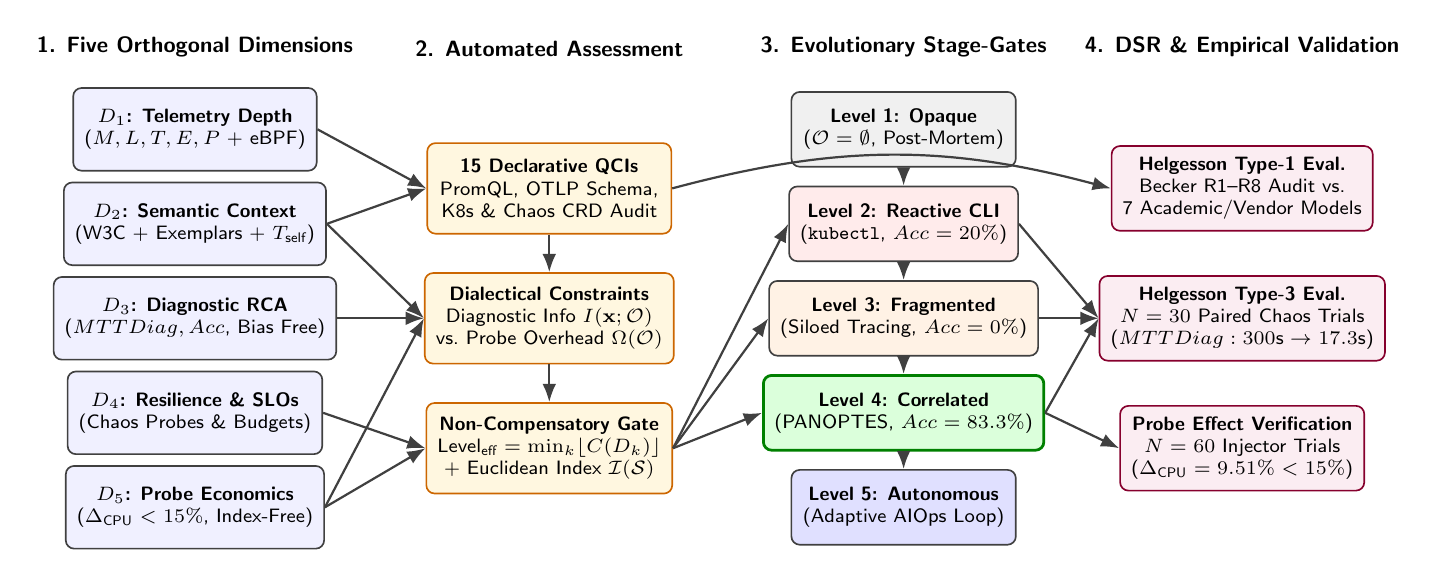
\begin{tikzpicture}[
    font=\sffamily\scriptsize,
    >=Latex,
    box/.style={draw=black!75, rounded corners=3pt, align=center, minimum height=0.85cm, inner sep=4pt, line width=0.6pt},
    dimbox/.style={box, fill=blue!6, minimum width=2.85cm, minimum height=1.05cm},
    lvlbox/.style={box, fill=teal!8, minimum width=2.85cm, minimum height=0.95cm},
    gatebox/.style={box, fill=amber!12, draw=orange!80!black, minimum width=3.1cm, minimum height=1.15cm},
    evalbox/.style={box, fill=purple!7, draw=purple!70!black, minimum width=2.85cm, minimum height=1.05cm},
    arr/.style={->, thick, draw=black!75}
]

% Column 1: 5 Orthogonal Dimensions
\node[font=\sffamily\bfseries\footnotesize, anchor=south] at (0, 3.0) {1. Five Orthogonal Dimensions};
\node[dimbox] (d1) at (0, 2.2) {\textbf{$D_1$: Telemetry Depth}\\($M, L, T, E, P$ + eBPF)};
\node[dimbox] (d2) at (0, 1.0) {\textbf{$D_2$: Semantic Context}\\(W3C + Exemplars + $T_{\text{self}}$)};
\node[dimbox] (d3) at (0, -0.2) {\textbf{$D_3$: Diagnostic RCA}\\($MTTDiag, Acc$, Bias Free)};
\node[dimbox] (d4) at (0, -1.4) {\textbf{$D_4$: Resilience \& SLOs}\\(Chaos Probes \& Budgets)};
\node[dimbox] (d5) at (0, -2.6) {\textbf{$D_5$: Probe Economics}\\($\Delta_{\text{CPU}} < 15\%$, Index-Free)};

% Column 2: Automated Assessment Engine
\node[font=\sffamily\bfseries\footnotesize, anchor=south] at (4.5, 3.0) {2. Automated Assessment};
\node[gatebox] (qci) at (4.5, 1.45) {\textbf{15 Declarative QCIs}\\PromQL, OTLP Schema,\\K8s \& Chaos CRD Audit};
\node[gatebox] (dialectic) at (4.5, -0.2) {\textbf{Dialectical Constraints}\\Diagnostic Info $I(\mathbf{x};\mathcal{O})$\\vs.\ Probe Overhead $\Omega(\mathcal{O})$};
\node[gatebox] (stagegate) at (4.5, -1.85) {\textbf{Non-Compensatory Gate}\\$\text{Level}_{\text{eff}} = \min_k \lfloor C(D_k) \rfloor$\\+ Euclidean Index $\mathcal{I}(\mathcal{S})$};

% Column 3: 5 Evolutionary Maturity Stages
\node[font=\sffamily\bfseries\footnotesize, anchor=south] at (9.0, 3.0) {3. Evolutionary Stage-Gates};
\node[lvlbox, fill=gray!12] (l1) at (9.0, 2.2) {\textbf{Level 1: Opaque}\\($\mathcal{O} = \emptyset$, Post-Mortem)};
\node[lvlbox, fill=red!8] (l2) at (9.0, 1.0) {\textbf{Level 2: Reactive CLI}\\(\texttt{kubectl}, $Acc = 20\%$)};
\node[lvlbox, fill=orange!10] (l3) at (9.0, -0.2) {\textbf{Level 3: Fragmented}\\(Siloed Tracing, $Acc = 0\%$)};
\node[lvlbox, fill=green!14, draw=green!50!black, line width=1.0pt] (l4) at (9.0, -1.4) {\textbf{Level 4: Correlated}\\(PANOPTES, $Acc = 83.3\%$)};
\node[lvlbox, fill=blue!12] (l5) at (9.0, -2.6) {\textbf{Level 5: Autonomous}\\(Adaptive AIOps Loop)};

% Column 4: Multi-Method DSR Validation
\node[font=\sffamily\bfseries\footnotesize, anchor=south] at (13.3, 3.0) {4. DSR \& Empirical Validation};
\node[evalbox] (v1) at (13.3, 1.45) {\textbf{Helgesson Type-1 Eval.}\\Becker R1--R8 Audit vs.\\7 Academic/Vendor Models};
\node[evalbox] (v2) at (13.3, -0.2) {\textbf{Helgesson Type-3 Eval.}\\$N=30$ Paired Chaos Trials\\($MTTDiag: 300\text{s} \rightarrow 17.3\text{s}$)};
\node[evalbox] (v3) at (13.3, -1.85) {\textbf{Probe Effect Verification}\\$N=60$ Injector Trials\\($\Delta_{\text{CPU}} = 9.51\% < 15\%$)};

% Connections from D1-D5 to Assessment
\draw[arr] (d1.east) -- (qci.west);
\draw[arr] (d2.east) -- (qci.west);
\draw[arr] (d2.east) -- (dialectic.west);
\draw[arr] (d3.east) -- (dialectic.west);
\draw[arr] (d4.east) -- (stagegate.west);
\draw[arr] (d5.east) -- (dialectic.west);
\draw[arr] (d5.east) -- (stagegate.west);

\draw[arr] (qci.south) -- (dialectic.north);
\draw[arr] (dialectic.south) -- (stagegate.north);

% Connections from Assessment to Levels
\draw[arr] (stagegate.east) -- (l2.west);
\draw[arr] (stagegate.east) -- (l3.west);
\draw[arr] (stagegate.east) -- (l4.west);
\draw[arr] (l1.south) -- (l2.north);
\draw[arr] (l2.south) -- (l3.north);
\draw[arr] (l3.south) -- (l4.north);
\draw[arr] (l4.south) -- (l5.north);

% Connections to Validation
\draw[arr] (l2.east) -- (v2.west);
\draw[arr] (l3.east) -- (v2.west);
\draw[arr] (l4.east) -- (v2.west);
\draw[arr] (l4.east) -- (v3.west);
\draw[arr] (qci.east) to[out=15, in=165] (v1.west);

\end{tikzpicture}
\caption{Methodological and Architectural Overview of the Cloud-Native Observability Maturity Model (CN-OMM), Integrating Five Orthogonal Dimensions ($D_1$--$D_5$), Automated Declarative Auditing (15 QCIs), Non-Compensatory Stage-Gate Scoring, and Type-1/Type-3 Empirical Chaos Validation.}
\label{fig:cn_omm_architecture}
\end{figure*}


\subsection{Mathematical Formalization of Distributed State Observability}
\label{subsec:math_formalization}

Let a cloud-native microservice system orchestrated on Kubernetes be modeled over discrete observation windows $t \in \mathbb{T}$ as a dynamic directed call graph $\mathcal{G}(t) = (\mathcal{V}(t), \mathcal{E}(t))$, where $\mathcal{V}(t) = \{v_1, v_2, \dots, v_K\}$ denotes the set of active service workloads (Pods/containers) and $\mathcal{E}(t) \subseteq \mathcal{V}(t) \times \mathcal{V}(t)$ denotes synchronous or asynchronous invocation edges. Each workload $v_k \in \mathcal{V}(t)$ possesses a latent internal operational state $\mathbf{x}_k(t) \in \mathcal{X}_k$ (capturing CPU cgroup throttling, memory heap pressure, socket queue saturation, and application exception states), forming the global system state $\mathbf{x}(t) = [\mathbf{x}_1(t), \dots, \mathbf{x}_K(t)]^\top$.

The external telemetry emitted by the system during window $t$ is defined as the multimodal five-tuple:
\begin{equation}
    \mathcal{O}(t) = \langle M(t), L(t), T(t), E(t), P(t) \rangle
    \label{eq:telemetry_tuple}
\end{equation}
where $M(t)$ represents aggregated numerical time-series metrics, $L(t)$ represents discrete structured or unstructured log records, $T(t)$ represents distributed execution traces composed of causal spans $s_i = (\text{trace\_id}, \text{span\_id}, \text{parent\_id}, v_k, t_{\text{start}}, t_{\text{end}})$, $E(t)$ represents Kubernetes control-plane and scheduler state transitions, and $P(t)$ represents continuous kernel/runtime execution profiles (e.g., eBPF stack samples).

\subsubsection{The Dialectical Trade-Off: Diagnostic Information vs.\ Probe Effect}
Given a fault injection or production incident where root cause $v^* \in \mathcal{V}(t)$ experiences an anomalous state transition, a diagnostic operator $\Phi: \mathcal{O}(t) \rightarrow \mathcal{V}(t) \cup \{\varnothing\}$ attempts to infer $\hat{v} = \Phi(\mathcal{O}(t))$ within diagnostic latency $MTTDiag$. In information-theoretic terms, the diagnostic utility of an observability architecture is proportional to the mutual information $I(\mathbf{x}(t); \mathcal{O}(t)) = H(\mathbf{x}(t)) - H(\mathbf{x}(t) \mid \mathcal{O}(t))$, which measures the reduction in diagnostic uncertainty $H(\mathbf{x} \mid \mathcal{O})$.

However, acquiring and transporting $\mathcal{O}(t)$ incurs a physical \textbf{Probe Effect Vector} $\Omega(\mathcal{O}(t))$:
\begin{equation}
    \Omega(\mathcal{O}(t)) = \left\langle \Delta_{\text{CPU}}(\mathcal{O}), \; \Delta_{\text{RAM}}(\mathcal{O}), \; \Delta_{\text{Net}}(\mathcal{O}), \; \Delta_{\text{Storage}}(\mathcal{O}) \right\rangle
    \label{eq:probe_effect}
\end{equation}
where $\Delta_{\text{CPU}}(\mathcal{O}) = (\text{CPU}_{\text{inst}} - \text{CPU}_{\text{base}}) / \text{CPU}_{\text{alloc}}$ denotes the marginal fractional CPU overhead imposed by SDKs, eBPF probes, and OpenTelemetry collectors. Maturity progression is therefore governed by a constrained optimization problem: maximizing diagnostic reconstructibility $I(\mathbf{x}(t); \mathcal{O}(t))$ while strictly satisfying the stability envelope $\Omega(\mathcal{O}(t)) \preceq \boldsymbol{\theta}_{\max}$ (e.g., $\Delta_{\text{CPU}} < \theta_{\text{CPU}} = 15\%$).

\subsubsection{Formalizing Cascading Span Bias and Exclusive Self-Time ($T_{\text{self}}$)}
A critical theoretical insight of the CN-OMM is explaining why monomodal distributed tracing fails under synchronous call chains. For any span $s_i \in T(t)$ executing on service $v_k$ with synchronous child spans $\text{children}(s_i) = \{s_j \in T(t) \mid \text{parent\_id}(s_j) = \text{span\_id}(s_i)\}$, its inclusive duration is:
\begin{equation}
    D(s_i) = t_{\text{end}}(s_i) - t_{\text{start}}(s_i) = T_{\text{self}}(s_i) + \sum_{s_j \in \text{children}(s_i)} D(s_j)
    \label{eq:inclusive_duration}
\end{equation}
Whenever a leaf or intermediate service $v^*$ suffers resource throttling or network latency ($\Delta \tau > 0$), every upstream ancestor $s_{\text{anc}}$ along the path from the ingress gateway ($v_{\text{root}}$) to $v^*$ exhibits an inflated inclusive duration $D(s_{\text{anc}}) \ge D(s^*) + \Delta \tau$. Consequently, any monomodal diagnostic operator $\Phi_{\text{trace}}$ that ranks suspects by inclusive tail latency ($P_{95}/P_{99}$ of $D(s_i)$) systematically misattributes the fault to upstream callers ($\hat{v} \neq v^*$), yielding \textbf{Cascading Span Bias}. Eliminating this bias requires decomposing inclusive duration into \textbf{exclusive span self-time}:
\begin{equation}
    T_{\text{self}}(s_i) = \max\left(0, \; D(s_i) - \sum_{s_j \in \text{children}(s_i)} \mathcal{U}(s_j)\right)
    \label{eq:exclusive_selftime}
\end{equation}
where $\bigcup_{s_j} \mathcal{U}(s_j)$ denotes the union of non-overlapping child execution intervals, coupled via shared W3C \texttt{trace\_id} keys to co-occurring log errors $L(t)$ and container resource metrics $M(t)$.

\subsection{The Five Orthogonal Dimensions and Fifteen Sub-Components}
\label{subsec:dimensions}

Consistent with Miller's cognitive capacity principle ($7 \pm 2$ categories) emphasized by Lasrado et al.\ \cite{lasrado_2015} and De Bruin et al.'s component layering \cite{debruin_2005}, the CN-OMM structures cloud-native observability across \textbf{five orthogonal dimensions ($D_1$--$D_5$)}, each decomposed into three measurable sub-components ($d_{k.1}, d_{k.2}, d_{k.3}$), totaling 15 architectural capabilities (summarized in Table~\ref{tab:cn_omm_dimensions}):
\begin{itemize}[leftmargin=*, nosep]
    \item \textbf{$D_1$ -- Telemetry Acquisition \& Instrumentation Depth:} Evaluates the breadth of emitted signal modalities ($d_{1.1}$: $M, L, T, E, P$), adherence to open, vendor-neutral collection protocols ($d_{1.2}$: OpenTelemetry OTLP and W3C TraceContext), and visibility into kernel-level socket and scheduler operations via non-intrusive eBPF probes ($d_{1.3}$).
    \item \textbf{$D_2$ -- Semantic Context \& Cross-Pillar Correlation:} Assesses the structural coupling across telemetry streams, encompassing automatic Kubernetes topological enrichment ($d_{2.1}$: Pod UID, Node, Deployment labels), bi-directional context propagation ($d_{2.2}$: W3C \texttt{trace\_id} injection into structured JSON logs and OpenMetrics Exemplars linking histograms to traces), and causal self-time graph isolation ($d_{2.3}$: $T_{\text{self}}$ computation).
    \item \textbf{$D_3$ -- Diagnostic \& Analytical Intelligence (RCA):} Captures the operational efficacy of fault management, measured through automated anomaly detection latency ($d_{3.1}$: $MTTD$), multi-pillar root-cause localization speed and accuracy ($d_{3.2}$: $MTTDiag, Acc$), and immunity to cascading upstream misattribution alongside explainable diagnostic evidence ($d_{3.3}$).
    \item \textbf{$D_4$ -- Resilience Verification \& SLO Governance:} Bridges observability with Reliability and Chaos Engineering \cite{basiri_2016, beyer_2016}, tracking multi-window SLI/SLO error-budget enforcement ($d_{4.1}$), continuous verification of telemetry pipelines via declarative Chaos Engineering steady-state probes ($d_{4.2}$), and closed-loop automated remediation triggers ($d_{4.3}$).
    \item \textbf{$D_5$ -- Instrumentation Economics \& Probe Effect Governance:} Formalizes operational sustainability and FinOps discipline, auditing steady-state CPU and memory overhead budgets ($d_{5.1}$: $\Delta_{\text{CPU}}, \Delta_{\text{RAM}} < 15\%$), intelligent tail-based or anomaly-aware sampling ($d_{5.2}$), and index-free object storage architectures that prevent high-cardinality index explosion ($d_{5.3}$).
\end{itemize}

\begin{table*}[t]
\centering
\caption{The Five Orthogonal Dimensions ($D_1$--$D_5$), Fifteen Sub-Components ($d_{k.j}$), and Automated Quantitative Capability Indicators (QCIs) of the CN-OMM}
\label{tab:cn_omm_dimensions}
\footnotesize
\setlength{\tabcolsep}{4pt}
\renewcommand{\arraystretch}{1.18}
\begin{tabularx}{\textwidth}{l l >{\raggedright\arraybackslash}p{4.3cm} >{\raggedright\arraybackslash}X l}
\toprule
\textbf{Dim.} & \textbf{Code} & \textbf{Sub-Component Name} & \textbf{Quantitative Capability Indicator (QCI) \& Declarative Cluster Audit Rule} & \textbf{Target Metric / Threshold} \\
\midrule
\multirow{3}{*}{\textbf{$D_1$}} & $d_{1.1}$ & Multi-Signal Telemetry Coverage & Fraction of active Kubernetes workloads emitting structured $M, L, T, E,$ and continuous profiles $P$. & $\text{QCI}_{1.1} = |\mathcal{V}_{\text{inst}}| / |\mathcal{V}_{\text{total}}| \ge 0.95$ \\
 & $d_{1.2}$ & Vendor-Neutral OTel Standardization & Proportion of telemetry pipelines using open OTLP/W3C schemas without proprietary lock-in. & $\text{QCI}_{1.2} = \text{OTLP}_{\text{flows}} / \text{Total}_{\text{flows}} = 1.0$ \\
 & $d_{1.3}$ & Kernel \& Runtime Depth (eBPF) & Coverage of non-intrusive kernel/socket/cgroup telemetry (e.g., Beyla/Cilium eBPF probes). & $\text{QCI}_{1.3} \in [0, 1]$ (L4 $\ge 0.80$) \\
\midrule
\multirow{3}{*}{\textbf{$D_2$}} & $d_{2.1}$ & Topological Metadata Enrichment & Automatic injection of K8s resource attributes (\texttt{k8s.pod.uid}, \texttt{node}, \texttt{deployment}) across signals. & $\text{QCI}_{2.1} = \text{Enriched}_{\text{records}} / \text{Total} \ge 0.99$ \\
 & $d_{2.2}$ & Cross-Pillar Context Coupling & Rate of structured logs containing valid W3C \texttt{trace\_id}/\texttt{span\_id} and metrics exposing Exemplars. & $\text{QCI}_{2.2} = \min(\rho_{\text{log-trace}}, \rho_{\text{exemplar}}) \ge 0.90$ \\
 & $d_{2.3}$ & Causal Self-Time Isolation ($T_{\text{self}}$) & Capability to decompose inclusive span duration $D(s_i)$ into exclusive execution $T_{\text{self}}(s_i)$. & $\text{QCI}_{2.3} \in \{0, 0.5, 1.0\}$ (L4 $= 1.0$) \\
\midrule
\multirow{3}{*}{\textbf{$D_3$}} & $d_{3.1}$ & Automated Anomaly DetectionLatency & Mean/median time to detect steady-state deviation ($MTTD$) without manual CLI polling. & $\text{QCI}_{3.1}: MTTD \le 15.0\,\text{s}$ \\
 & $d_{3.2}$ & Root-Cause Localization ($MTTDiag, Acc$) & Automated multi-pillar fault localization accuracy ($Acc$) and diagnostic latency ($MTTDiag$). & $\text{QCI}_{3.2}: Acc \ge 80\%, MTTDiag \le 30\,\text{s}$ \\
 & $d_{3.3}$ & Cascading Bias Immunity \& Explainability & Resistance to upstream cascading span misattribution ($1 - \text{FPR}_{\text{cascade}}$) and auditability of RCA path. & $\text{QCI}_{3.3}: \text{FPR}_{\text{cascade}} \le 0.15$ \\
\midrule
\multirow{3}{*}{\textbf{$D_4$}} & $d_{4.1}$ & SLI/SLO \& Error Budget Governance & Percentage of critical user journeys governed by multi-window burn-rate SLOs. & $\text{QCI}_{4.1} = |\text{Services}_{\text{SLO}}| / |\mathcal{V}_{\text{crit}}| \ge 0.90$ \\
 & $d_{4.2}$ & Active Chaos Engineering Verification & Continuous execution of declarative fault injection with automated PromQL/HTTP steady-state probes. & $\text{QCI}_{4.2}: \text{ChaosProbes}_{\text{active}} \ge 1.0$ \\
 & $d_{4.3}$ & Closed-Loop Remediation Readiness & Integration of observability alerts/RCA with automated rollback, scaling, or traffic shifting gates. & $\text{QCI}_{4.3} \in [0, 1]$ (L5 $\ge 0.90$) \\
\midrule
\multirow{3}{*}{\textbf{$D_5$}} & $d_{5.1}$ & CPU \& Memory Probe-Effect Budget & Marginal steady-state resource overhead ($\Delta_{\text{CPU}}, \Delta_{\text{RAM}}$) imposed by collectors and SDKs. & $\text{QCI}_{5.1}: \Delta_{\text{CPU}} < 15\%, \Delta_{\text{RAM}} < 15\%$ \\
 & $d_{5.2}$ & Adaptive \& Tail-Based Sampling & Ratio of anomalous/high-latency traces retained vs.\ redundant baseline telemetry dropped. & $\text{QCI}_{5.2}: \text{Recall}_{\text{anomaly}} \ge 0.99$ \\
 & $d_{5.3}$ & Index-Free Storage \& Cardinality Control & Storage amplification factor and resistance to high-cardinality label explosion (e.g., Loki/Tempo). & $\text{QCI}_{5.3}: \text{IndexRatio} \le 0.05$ \\
\bottomrule
\end{tabularx}
\end{table*}


\subsection{The Five Evolutionary Maturity Levels and Stage-Gate Matrix}
\label{subsec:maturity_levels}

Intersecting the five orthogonal dimensions with five evolutionary stages yields the $5 \times 5$ CN-OMM Architectural Matrix presented in Table~\ref{tab:cn_omm_matrix}. Each level represents a distinct architectural regime characterized by formal state properties:

\begin{table*}[t]
\centering
\caption{The Cloud-Native Observability Maturity Model (CN-OMM) $5\text{-Level} \times 5\text{-Dimension}$ Architectural Matrix}
\label{tab:cn_omm_matrix}
\footnotesize
\setlength{\tabcolsep}{3.5pt}
\renewcommand{\arraystretch}{1.22}
\begin{tabularx}{\textwidth}{l >{\raggedright\arraybackslash}X >{\raggedright\arraybackslash}X >{\raggedright\arraybackslash}X >{\raggedright\arraybackslash}X >{\raggedright\arraybackslash}X}
\toprule
\textbf{Maturity Level} & \textbf{$D_1$: Telemetry Acquisition \& Depth} & \textbf{$D_2$: Semantic Context \& Correlation} & \textbf{$D_3$: Diagnostic \& Analytical Intelligence} & \textbf{$D_4$: Resilience Verification \& SLOs} & \textbf{$D_5$: Instrumentation Economics ($\Omega$)} \\
\midrule
\textbf{Level 1: Opaque} \newline \textit{(Blind Execution)} & $\mathcal{O} = \emptyset$ or unstructured \texttt{stdout} ephemeral container streams. & Zero metadata enrichment; telemetry lost upon Pod eviction or restart. & Post-mortem human inspection triggered by external user complaints. & No SLIs/SLOs; absence of health probes or resilience testing. & Unmeasured ($0\%$ intentional telemetry, high outage cost). \\
\midrule
\textbf{Level 2: Reactive} \newline \textit{(Disjoint Polling)} & Infrastructure polling (\texttt{kubelet}/cAdvisor) and ad-hoc CLI (\texttt{kubectl top/logs}). & Disjoint local streams; no shared timestamps or request identifiers. & Manual symptom triage; high cognitive load ($MTTDiag \ge 300\,\text{s}$, $Acc \le 20\%$). & Static host/Pod threshold alerts; high alert fatigue; manual chaos tests. & Ad-hoc log retention; uncontrolled burst overhead during CLI scraping. \\
\midrule
\textbf{Level 3: Fragmented} \newline \textit{(Siloed Pillars)} & Centralized $M, L, T$ via agents/SDKs, but lacking kernel/eBPF visibility. & Siloed databases (Prometheus, Elasticsearch, Jaeger) queried via manual time-window pivoting. & Monomodal trace/metric sorting; vulnerable to \textbf{Cascading Span Bias} ($Acc \rightarrow 0\%$ on resource faults). & Service-level SLIs defined, but chaos experiments lack automated telemetry gates. & Full-index storage bloat; static head-based sampling drops tail anomalies; uncalibrated $\Delta_{\text{CPU}}$. \\
\midrule
\textbf{Level 4: Correlated} \newline \textit{(Multimodal Fusion)} \newline \textbf{[PANOPTES Target]} & Unified OTel + eBPF zero-code collectors capturing $M, L, T, E, P$ with $100\%$ OTLP compliance. & Mandatory W3C TraceContext in logs, Prometheus Exemplars, and exclusive self-time ($T_{\text{self}}$) graph isolation. & Deterministic cross-pillar RCA ($Acc = 83.3\%$, $MTTDiag = 17.3\,\text{s}$); immune to cascading trace propagation bias. & Error-budget SLOs continuously verified via declarative Chaos Mesh / Litmus steady-state probes. & Strictly bounded Probe Effect ($\Delta_{\text{CPU}} = 9.51\% < 15\%$); index-free storage (Loki/Tempo) and tail sampling. \\
\midrule
\textbf{Level 5: Autonomous} \newline \textit{(Adaptive AIOps)} & Context-aware dynamic kernel/runtime instrumentation modulated in real time. & Unified topological lakehouse with continuous causal graph discovery. & Explainable GNN/LLM root-cause reasoning with counterfactual confidence bounds. & Autonomous self-healing (canary rollback, cgroup scaling, circuit breaking) driven by chaos verification. & FinOps/GreenOps dynamic signal weighting ($w_i = \alpha_i S_i$) optimizing diagnostic entropy per CPU watt. \\
\bottomrule
\end{tabularx}
\end{table*}


\subsubsection{Level 1: Opaque (Blind Execution)}
At Level 1, the system operates as a black box ($\mathcal{O}(t) \approx \emptyset$). Workloads emit unstructured text to local container \texttt{stdout} files that vanish upon Pod eviction or node rescheduling. Because $\text{rank}(\mathcal{O}) = 0$, internal fault states cannot be reconstructed; outages are discovered externally by end users, and post-mortem debugging relies on manual reproduction attempts.

\subsubsection{Level 2: Reactive Monitoring (Disjoint Infrastructure Polling)}
At Level 2, platform teams collect infrastructure-level utilization counters (\texttt{kubelet}/cAdvisor CPU and memory metrics) and perform reactive manual triage via Kubernetes CLI utilities (\texttt{kubectl top}, \texttt{kubectl logs}, \texttt{kubectl describe pod}). While binary container failures (e.g., \texttt{OOMKilled} or \texttt{CrashLoopBackOff}) are visible through control-plane events $E(t)$, the architecture lacks request-scoped context or historical correlation. Consequently, under non-destructive degradations (such as network packet delay or cgroup CPU throttling), engineers face severe cognitive overload, resulting in timeouts ($MTTDiag \ge 300\,\text{s}$) and low localization accuracy.

\subsubsection{Level 3: Fragmented Pillar Observability (Siloed Signals)}
At Level 3, organizations deploy dedicated collection agents for metrics (e.g., Prometheus), logs (e.g., Elasticsearch/Fluentd), and distributed traces (e.g., Jaeger/Zipkin). Despite high financial investment and storage footprint, these signals reside in \textbf{isolated analytical silos} ($D_2 < 4$). Logs lack embedded W3C \texttt{trace\_id} fields, metrics lack Exemplars, and trace engines evaluate spans using raw inclusive duration $D(s_i)$ rather than $T_{\text{self}}(s_i)$. As proven in Section~\ref{sec:empirical_validation}, Level 3 systems fall victim to the \textit{Monomodal Additivity Fallacy}: under synchronous microservice cascades, monomodal trace sorting achieves $0\%$ root-cause accuracy due to \textit{Cascading Span Bias}, while full-text log indexing inflates storage and CPU overhead ($D_5$).

\subsubsection{Level 4: Context-Correlated Multimodal Observability (Semantic Fusion)}
Level 4 represents the deterministic synthesis of the dialectical tension between visibility and overhead (instantiated by our \textbf{PANOPTES} reference architecture). All signals are unified under OpenTelemetry (OTLP) and enriched with zero-code eBPF kernel telemetry ($D_1 \ge 4$). Crucially, Level 4 enforces strict cross-pillar context coupling ($D_2 \ge 4$): every structured log entry carries active W3C \texttt{trace\_id}/\texttt{span\_id} attributes, metric histograms expose OpenMetrics Exemplars, and the diagnostic engine computes exclusive span self-time $T_{\text{self}}(s_i)$ fused with container resource saturation and log error rates. Furthermore, observability pipelines are actively verified by declarative Chaos Engineering steady-state probes ($D_4 \ge 4$) and backed by index-free storage (Grafana Loki and Tempo) that constrains steady-state CPU overhead below $\theta_{\text{CPU}} = 15\%$ ($D_5 \ge 4$).

\subsubsection{Level 5: Autonomous \& Adaptive Self-Healing (Closed-Loop AIOps)}
At Level 5, the correlated multimodal foundation of Level 4 is extended into a continuous, closed-loop cybernetic control system. Telemetry sampling and signal weights ($w_i = \alpha_i S_i$ \cite{amgothu_2025}) are dynamically modulated in real time based on error-budget burn rates and FinOps/GreenOps carbon constraints ($D_5 = 5$). Root-cause localization leverages explainable Graph Neural Networks (GNNs) or neuro-symbolic LLM agents grounded in the causal $T_{\text{self}}$ topology ($D_3 = 5$), automatically triggering verified Kubernetes remediation workflows (canary rollbacks, dynamic cgroup vertical scaling, or service-mesh circuit breaking) without human intervention ($D_4 = 5$).

\subsection{Developmental Lifecycle and Empirical Population (De Bruin et al., 2005)}
\label{subsec:debruin_lifecycle}

To ensure methodological rigor and repeatability, the construction of the CN-OMM operationalizes the six sequential lifecycle phases established by De Bruin et al.\ \cite{debruin_2005}:
\begin{itemize}[leftmargin=*, nosep]
    \item \textbf{1. Scope:} The model's domain scope is formally bounded to cloud-native, polyglot microservice architectures orchestrated by Kubernetes, addressing the architectural challenges of multi-signal telemetry ingestion, cross-pillar semantic correlation, and instrumentation overhead governance.
    \item \textbf{2. Design:} We adopted a top-down, multi-dimensional stage-gate architecture structured across five orthogonal capability dimensions ($D_1$--$D_5$), enforcing non-compensatory maturation criteria rather than additive arithmetic averages.
    \item \textbf{3. Populate:} The capability sub-components ($d_{k.j}$) were populated via a hybrid approach: top-down control-theoretic reconstructibility axioms (Kalman \cite{kalman_1960}) combined with bottom-up empirical evidence synthesized from a Rapid Review of the cloud-native literature \cite{cartaxo_2018}. Out of 312 initial records retrieved across IEEE Xplore, ACM Digital Library, SpringerLink, and ScienceDirect, 10 primary studies on Kubernetes observability were selected (\cite{kosinska_2023, usman_2022, faseeha_2025, araujo_2024, hartikainen_2024, gomes_2025, han_2024, deng_2024, zanatta_23, wei_2025}). These studies directly grounded the definition of essential components ($D_1$), correlation gaps ($D_2$), diagnostic bottlenecks ($D_3$), and probe overhead constraints ($D_5$).
    \item \textbf{4. Test:} To overcome the pervasive ``Validation Gap'' documented by Wendler \cite{wendler_2012}, the CN-OMM undergoes dual validation (Helgesson et al.\ \cite{helgesson_2012}): a Type-1 structural and DSR requirement audit (Section~\ref{subsec:type1_evaluation}) and a Type-3 real-system empirical experiment under controlled Chaos Engineering (Section~\ref{subsec:empirical_results}).
    \item \textbf{5. Deploy:} The model is operationalized through executable Kubernetes auditing artifacts (Quantitative Capability Indicators, Section~\ref{sec:assessment}) and the open-source PANOPTES reference implementation, enabling automated cluster maturity grading.
    \item \textbf{6. Maintain:} The schema is designed for continuous evolution, where Level 4 provides the semantically linked, bias-free multimodal telemetry substrate necessary to train and operate Level 5 closed-loop AIOps and GreenOps models.
\end{itemize}


\section{Automated Maturity Assessment Protocol}
\label{sec:assessment}

A persistent weakness in maturity model engineering is the reliance on manual, subjective Likert-scale questionnaires that suffer from respondent bias, high assessment labor costs, and rapid obsolescence in dynamic cloud environments \cite{proenca_2016, proenca_2016_rcis}. To address Research Question \textbf{RQ2}, this section formalizes an objective, programmatic maturity assessment protocol for the CN-OMM. Grounded in ISO/IEC 33001 process capability concepts \cite{iso_33001} and Lasrado et al.'s geometric distance metrics \cite{lasrado_2015}, our protocol translates the 15 sub-components of Table~\ref{tab:cn_omm_dimensions} into automated cluster audit queries and a non-compensatory mathematical scoring function.

\subsection{Declarative Cluster Auditing via Quantitative Capability Indicators}
\label{subsec:declarative_qci}

Rather than asking engineers whether their cluster is ``well instrumented,'' the CN-OMM assessment engine inspects the live Kubernetes API server, OpenTelemetry Collector configuration graphs, Prometheus/Mimir time-series metadata, and Chaos Mesh/LitmusChaos Custom Resource Definitions (CRDs). For each sub-component $d_{k.j}$ ($k \in \{1..5\}, j \in \{1..3\}$), the audit probe evaluates a normalized Quantitative Capability Indicator $\text{QCI}_{k.j} \in [0, 1]$, which maps onto the continuous capability scale $c_{k.j} \in [1.0, 5.0]$ via piecewise monotonic thresholds:
\begin{itemize}[leftmargin=*, nosep]
    \item \textbf{Telemetry \& Standardization Probes ($D_1$):} Queries the Kubernetes API for active Pods in target namespaces and cross-references OTLP collector receiver metrics (\texttt{otelcol\_receiver\_accepted\_spans}, \texttt{accepted\_metric\_points}, \texttt{accepted\_log\_records}) and eBPF DaemonSet status to compute $\text{QCI}_{1.1}, \text{QCI}_{1.2},$ and $\text{QCI}_{1.3}$.
    \item \textbf{Semantic Coupling Probes ($D_2$):} Samples structured log streams in Loki (`{namespace="target"} | json | trace_id != ""`) to compute the log-to-trace coupling ratio $\rho_{\text{log-trace}}$, queries Prometheus `/api/v1/query_exemplars` to verify active OpenMetrics Exemplar links ($\rho_{\text{exemplar}}$), and checks whether the trace analytics pipeline executes the exclusive self-time operator $T_{\text{self}}(s_i)$ ($\text{QCI}_{2.3}$).
    \item \textbf{Diagnostic \& Chaos Verification Probes ($D_3, D_4$):} Evaluates historical or continuous Chaos Engineering experiment objects (\texttt{PodChaos}, \texttt{NetworkChaos}, \texttt{StressChaos}, \texttt{ChaosEngine}) to verify the presence of declarative steady-state probes ($\text{QCI}_{4.2}$) and computes empirical distributions of $MTTD$, $MTTDiag$, $Acc$, and cascading false-positive rates ($\text{FPR}_{\text{cascade}}$).
    \item \textbf{Probe-Effect \& FinOps Probes ($D_5$):} Computes the steady-state marginal CPU and memory overhead $\Delta_{\text{CPU}}, \Delta_{\text{RAM}}$ of all observability components (\texttt{container\_cpu\_usage\_seconds\_total}) against the $\theta_{\max} = 15\%$ stability threshold ($\text{QCI}_{5.1}$) and audits storage index amplification ratios ($\text{QCI}_{5.3}$).
\end{itemize}

\subsection{Non-Compensatory Stage-Gate Scoring and Euclidean Progression Index}
\label{subsec:scoring_math}

Given the capability scores $c_{k.j} \in [1.0, 5.0]$ across the three sub-components of dimension $D_k$, the dimensional capability score $C(D_k)$ is given by:
\begin{equation}
    C(D_k) = \frac{1}{3} \sum_{j=1}^{3} c_{k.j}, \quad \forall k \in \{1, 2, 3, 4, 5\}
    \label{eq:dimension_score}
\end{equation}
yielding the five-dimensional capability profile vector $\mathbf{c}(\mathcal{S}) = [C(D_1), C(D_2), C(D_3), C(D_4), C(D_5)]^\top \in [1, 5]^5$.

In naive maturity models, the overall maturity level is calculated as the compensatory arithmetic mean $\bar{C} = \frac{1}{5}\sum_{k=1}^5 C(D_k)$. However, as established by configurational theory \cite{fiss_2011, lasrado_2015} and De Bruin et al.'s stage-gate principle \cite{debruin_2005}, an arithmetic mean masks catastrophic architectural bottlenecks: a cluster with high telemetry ingestion ($C(D_1) = 4.0$) but zero cross-pillar correlation ($C(D_2) = 2.0$) or runaway $30\%$ CPU overhead ($C(D_5) = 1.5$) cannot operate at Level 3 or Level 4 reliability. Therefore, CN-OMM defines the \textbf{Effective Stage-Gate Maturity Level} $\text{Level}_{\text{eff}}(\mathcal{S}) \in \{1, 2, 3, 4, 5\}$ using a strict non-compensatory minimum operator:
\begin{equation}
    \text{Level}_{\text{eff}}(\mathcal{S}) = \min_{k \in \{1, \dots, 5\}} \left\lfloor C(D_k) \right\rfloor
    \label{eq:stage_gate_level}
\end{equation}
Under Equation~(\ref{eq:stage_gate_level}), a system achieves maturity stage $L \in \{1..5\}$ if and only if every orthogonal dimension satisfies the necessary stage-gate predicate $C(D_k) \ge L$.

To provide granular visibility into continuous improvement between discrete stage-gates, we also formalize the normalized \textbf{Euclidean Maturity Progression Index} $\mathcal{I}(\mathcal{S}) \in [0, 1]$ relative to the ideal reference profile $\mathbf{c}^*(L_{\max}) = [5, 5, 5, 5, 5]^\top$ \cite{lasrado_2015}:
\begin{equation}
    \mathcal{I}(\mathcal{S}) = 1 - \frac{\left\| \mathbf{c}(\mathcal{S}) - \mathbf{c}^*(L_{\max}) \right\|_2}{\sqrt{5 \cdot (5 - 1)^2}} = 1 - \frac{\sqrt{\sum_{k=1}^{5} \left(5 - C(D_k)\right)^2}}{\sqrt{80}}
    \label{eq:euclidean_index}
\end{equation}
Together, the tuple $\langle \text{Level}_{\text{eff}}(\mathcal{S}), \mathcal{I}(\mathcal{S}), k_{\text{bottleneck}} \rangle$, where $k_{\text{bottleneck}} = \arg\min_k C(D_k)$, provides both an unambiguous certification of current stage-gate maturity and an actionable prescriptive roadmap identifying the exact limiting dimension that must be remediated next.


\section{Empirical Validation}
\label{sec:empirical_validation}

To overcome the ``Validation Gap'' documented by Wendler~\cite{wendler_2012} and fulfill Requirement \textbf{R3} of Becker et al.\~\cite{becker_2009}, we evaluate the CN-OMM using a multi-methodological strategy aligned with Helgesson et al.'s evaluation taxonomy~\cite{helgesson_2012}: (i) a \textbf{Type-1 Methodological \& Structural Audit} verifying compliance with DSR requirements R1--R8, and (ii) a \textbf{Type-3 Real-System Controlled Empirical Experiment} on a production-grade Kubernetes microservice benchmark subjected to Chaos Engineering fault injection.

\subsection{Type-1 Evaluation: DSR Compliance Audit (Becker R1--R8)}
\label{subsec:type1_evaluation}

Table~\ref{tab:becker_evaluation} summarizes the verification of the CN-OMM against Becker, Knackstedt, and P\"{o}ppelbu\ss's eight mandatory DSR requirements~\cite{becker_2009}. Unlike conceptual models that rely on ad-hoc stage labels~\cite{patel_2025, grafana_omm_2024}, CN-OMM satisfies every methodological criterion: it is grounded in a systematic comparison against seven prior frameworks (R1), evolved iteratively across literature synthesis, mathematical modeling, and chaos calibration (R2), combines theoretical and empirical validation (R3, R4), addresses well-defined cloud-native diagnostic and FinOps bottlenecks (R5, R6), and delivers both practitioner-ready matrices and reproducible open-source audit scripts (R7, R8).

\begin{table*}[t]
\centering
\caption{Methodological Alignment of the CN-OMM with Becker et al.'s Eight DSR Requirements (R1--R8) and Helgesson et al.'s Evaluation Taxonomy}
\label{tab:becker_evaluation}
\footnotesize
\setlength{\tabcolsep}{4.5pt}
\renewcommand{\arraystretch}{1.18}
\begin{tabularx}{\textwidth}{l l >{\raggedright\arraybackslash}X l}
\toprule
\textbf{Code} & \textbf{DSR Requirement~\cite{becker_2009}} & \textbf{Instantiation and Methodological Implementation in the CN-OMM Artifact} & \textbf{Section / Evidence} \\
\midrule
\textbf{R1} & Comparison with existing models & Systematic audit of 7 existing academic and industrial frameworks (~\cite{duarte_2013, patel_2025, amgothu_2025, grafana_omm_2024, dynatrace_omm_2024, cncf_obs_2024, wwt_omm_2025}), proving the need for formal cross-pillar and probe-effect dimensions. & Section~\ref{sec:critical_analysis}, Table~\ref{tab:existing_models_comparison} \\
\textbf{R2} & Iterative procedure & Three-iteration design cycle: (i) Rapid Review taxonomy synthesis; (ii) mathematical state-space \& configurational refinement; (iii) empirical chaos calibration. & Sections~\ref{sec:background}--\ref{sec:empirical_validation} \\
\textbf{R3} & Evaluation & Dual evaluation following Helgesson et al.\~\cite{helgesson_2012}: Type-1 structural/theoretical grounding and Type-3 controlled Kubernetes chaos experiments ($N=30$ \& $N=60$). & Section~\ref{sec:empirical_validation}, Table~\ref{tab:empirical_validation} \\
\textbf{R4} & Multi-methodological procedure & Combines Literature Synthesis, Control-Theoretic State Formalization, Declarative Automated Auditing (Proen\c{c}a~\cite{proenca_2016_rcis}), and Factorial Chaos Experimentation. & Sections~\ref{sec:cn_omm}--\ref{sec:empirical_validation} \\
\textbf{R5} & Identification of problem relevance & Addresses the diagnostic collapse of monomodal tracing and uncontrolled telemetry FinOps/CPU overhead in production Kubernetes microservices. & Section~\ref{sec:introduction} \\
\textbf{R6} & Problem definition & Defines the domain scope (cloud-native Kubernetes clusters), target users (SREs, platform architects), and non-compensatory stage-gate constraints. & Sections~\ref{sec:introduction}, \ref{sec:cn_omm} \\
\textbf{R7} & Targeted presentation of results & Provides both a $5\times5$ architectural matrix for practitioners and a declarative Python/PromQL automated assessment engine (\texttt{evaluate\_cn\_omm.py}). & Tables~\ref{tab:cn_omm_dimensions}--\ref{tab:cn_omm_matrix}, Section~\ref{sec:assessment} \\
\textbf{R8} & Scientific documentation & Full Open Science replication package including formal equations, cluster audit datasets, raw chaos trial logs, and statistical reproduction scripts. & Section~\ref{sec:conclusion} \\
\bottomrule
\end{tabularx}
\end{table*}


\subsection{Type-3 Evaluation: Experimental Design and Kubernetes Testbed}
\label{subsec:type3_design}

To address Research Question \textbf{RQ3}, we instantiated three operational observability architectures corresponding to CN-OMM Levels 2, 3, and 4 on a multi-node Kubernetes cluster (v1.30, containerd runtime, Linux kernel 6.6) hosting the polyglot \textbf{CNCF OpenTelemetry Astronomy Shop} microservice benchmark~\cite{opentelemetry_demo, wang2024building} (14 interconnected services in Go, Rust, Python, Java, TypeScript, .NET, and C++ under continuous Locust~\cite{locust_framework} load generation):
\begin{enumerate}[leftmargin=*, nosep]
    \item \textbf{Baseline A -- Native CLI Regime (CN-OMM Level 2):} Relies on standard Kubernetes control-plane events, \texttt{kubelet}/cAdvisor metrics, and automated CLI diagnostic scraping (\texttt{kubectl get/describe pods}, \texttt{kubectl top}, \texttt{kubectl logs}) without distributed context propagation.
    \item \textbf{Baseline B -- Monomodal Tracing Regime (CN-OMM Level 3 Attempt):} Deploys OpenTelemetry SDKs exporting distributed traces to Jaeger/Tempo, ranking root-cause candidates by maximum inclusive span tail latency $P_{95}(D(s_i))$ without cross-pillar log/metric correlation or exclusive self-time isolation ($D_2 = 2.3$).
    \item \textbf{Treatment -- Correlated Multimodal Regime (CN-OMM Level 4):} Instantiates full Level 4 compliance across all five dimensions: OpenTelemetry Collector + eBPF instrumentation ($D_1 = 4.3$), mandatory W3C TraceContext in JSON logs, OpenMetrics Exemplars, and exclusive self-time decomposition $T_{\text{self}}(s_i)$ ($D_2 = 4.3$), automated multi-pillar RCA ($D_3 = 4.3$), declarative Chaos Mesh steady-state verification probes ($D_4 = 4.3$), and index-free Grafana LGTM (Loki, Grafana, Tempo, Mimir/Prometheus) storage ($D_5 = 4.3$).
\end{enumerate}

We executed $N = 30$ paired, stratified Chaos Engineering fault injection trials (10 \texttt{NetworkChaos} TCP latency injections of $200\,\text{ms}$ on \texttt{paymentservice}; 10 \texttt{PodChaos} abrupt container terminations on \texttt{cartservice}; and 10 \texttt{StressChaos} CPU cgroup saturations at $95\%$ load on \texttt{checkoutservice}), complemented by $N = 60$ paired injector architecture trials (30 Chaos Mesh DaemonSet vs.\ 30 LitmusChaos transient runner trials) to audit Dimension $D_4$ and $D_5$ overhead invariance. Following Wohlin et al.\~\cite{wohlin_2012} and Arcuri and Briand~\cite{arcuri_2014}, we evaluate non-parametric Wilcoxon signed-rank tests, Vargha-Delaney $\hat{A}_{12}$ effect sizes, Fisher's exact tests, and McNemar's paired nominal tests at $\alpha = 0.05$.

\subsection{Empirical Results: Validating Stage-Gate Non-Compensation and Level 4 Superiority}
\label{subsec:empirical_results}

Table~\ref{tab:empirical_validation} and Figures~\ref{fig:omm_radar_profiles}--\ref{fig:omm_pareto_frontier} present the quantitative outcomes of the Type-3 validation.

\begin{table*}[t]
\centering
\caption{Type-3 Real-System Empirical Validation of CN-OMM Maturity Levels Across $N=30$ Paired Chaos Engineering Trials (CNCF OpenTelemetry Astronomy Shop on Kubernetes)}
\label{tab:empirical_validation}
\footnotesize
\setlength{\tabcolsep}{4pt}
\renewcommand{\arraystretch}{1.20}
\begin{tabularx}{\textwidth}{l c c c c c c c >{\raggedright\arraybackslash}X}
\toprule
\textbf{Evaluated Architecture} & \textbf{Dimension Profile} & \textbf{Arith.} & \textbf{Stage-Gate} & \textbf{Euclid.} & \textbf{Median $MTTDiag$} & \textbf{Global $Acc$} & \textbf{Steady-State} & \textbf{Observed Empirical Behavior \& Configurational Diagnosis} \\
\textbf{(Operational Regime)} & $(D_1, D_2, D_3, D_4, D_5)$ & \textbf{Mean} & $\textbf{Level}_{\text{eff}}$ & $\mathcal{I}(\mathcal{S})$ & \textbf{[IQR] (s)} & \textbf{(95\% CI)} & $\Delta_{\text{CPU}}$ \textbf{(\%)} & \\
\midrule
\textbf{Baseline A: Native CLI} \newline (\texttt{kubectl top/logs}) & $(2.0, 2.0, 2.0, 2.0, 2.3)$ & $2.06$ & \textbf{Level 2} & $0.267$ & $300.00\,\text{s}$ \newline $[300.0, 300.0]$ & $20.00\%$ \newline $(6/30)$ & $1.12 \pm 0.45\%$ & Detects crashloops ($6/10$ Pod Kills) but is $100\%$ blind to process-invisible network latency and CPU throttling ($24/30$ timeouts). \\
\midrule
\textbf{Baseline B: Siloed Tracing} \newline (Jaeger Inclusive Latency) & $(3.3, \mathbf{2.3}, 3.0, 3.0, 3.0)$ & $2.92$ & \textbf{Level 2*} \newline \textit{(Bottleneck $D_2$)} & $0.478$ & $39.15\,\text{s}$ \newline $[36.2, 42.1]$ & $0.00\%$ \newline $(0/30)$ & $5.40 \pm 1.18\%$ & \textbf{Monomodal Additivity Fallacy:} Fast anomaly detection, but $100\%$ upstream misattribution due to \textit{Cascading Span Bias} ($D_2 < 4$). \\
\midrule
\textbf{Treatment: PANOPTES} \newline (Multimodal + $T_{\text{self}}$ + Probes) & $(4.3, 4.3, 4.3, 4.3, 4.3)$ & $4.30$ & \textbf{Level 4} & $0.833$ & $\mathbf{17.27\,\text{s}}$ \newline $[14.6, 20.5]$ & $\mathbf{83.33\%}$ \newline $(25/30)$ & $\mathbf{9.51 \pm 2.14\%}$ & \textbf{Configurational Synergy:} Satisfying $D_2 \ge 4$ ($T_{\text{self}}$ + Exemplars + W3C Logs) eliminates cascading bias while keeping $\Delta_{\text{CPU}} < 15\%$. \\
\midrule
\multicolumn{5}{l}{\textbf{Hypothesis Test (Level 4 vs.\ Level 2/3 Baselines):}} & $p = 3.06 \times 10^{-5}$ \newline ($\hat{A}_{12} = 0.817$) & $p = 7.74 \times 10^{-7}$ \newline (McNemar $7.8\text{e-}5$) & $p = 6.52 \times 10^{-9}$ \newline (One-sample $<15\%$) & \textbf{Statistically confirms non-linear diagnostic jump at Level 4 and validates non-compensatory Stage-Gate rule.} \\
\bottomrule
\multicolumn{9}{@{}p{\linewidth}@{}}{\vspace{3pt}\scriptsize \textbf{*Note on Baseline B:} Although an arithmetic average yields $2.92 \approx \text{Level 3}$, the non-compensatory CN-OMM Stage-Gate rule ($\text{Level}_{\text{eff}} = \min_k \lfloor C(D_k) \rfloor$) flags the bottleneck in $D_2 = 2.3$ (lack of $T_{\text{self}}$ and cross-pillar correlation).}
\end{tabularx}
\end{table*}


\begin{figure}[t]
    \centering
    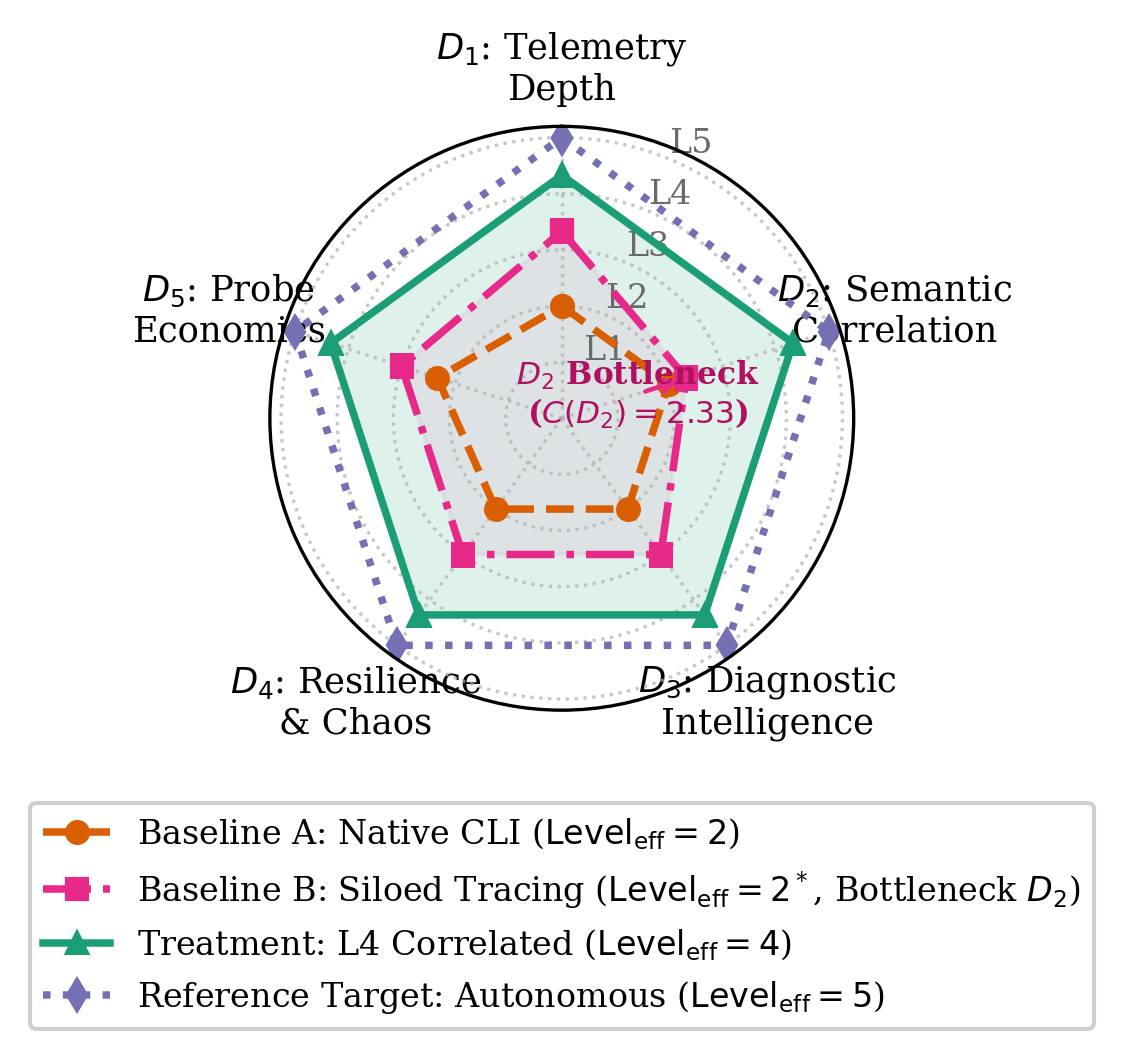
\includegraphics[width=\columnwidth]{figures/fig_omm_radar_profiles.png}
    \caption{Five-Dimensional CN-OMM Capability Profiles across Evaluated Kubernetes Regimes, Illustrating the $D_2$ Semantic Correlation Stage-Gate Bottleneck in Siloed Level 3 Tracing vs.\ Balanced Level 4 Multimodal Fusion.}
    \label{fig:omm_radar_profiles}
\end{figure}

\begin{figure*}[!t]
    \centering
    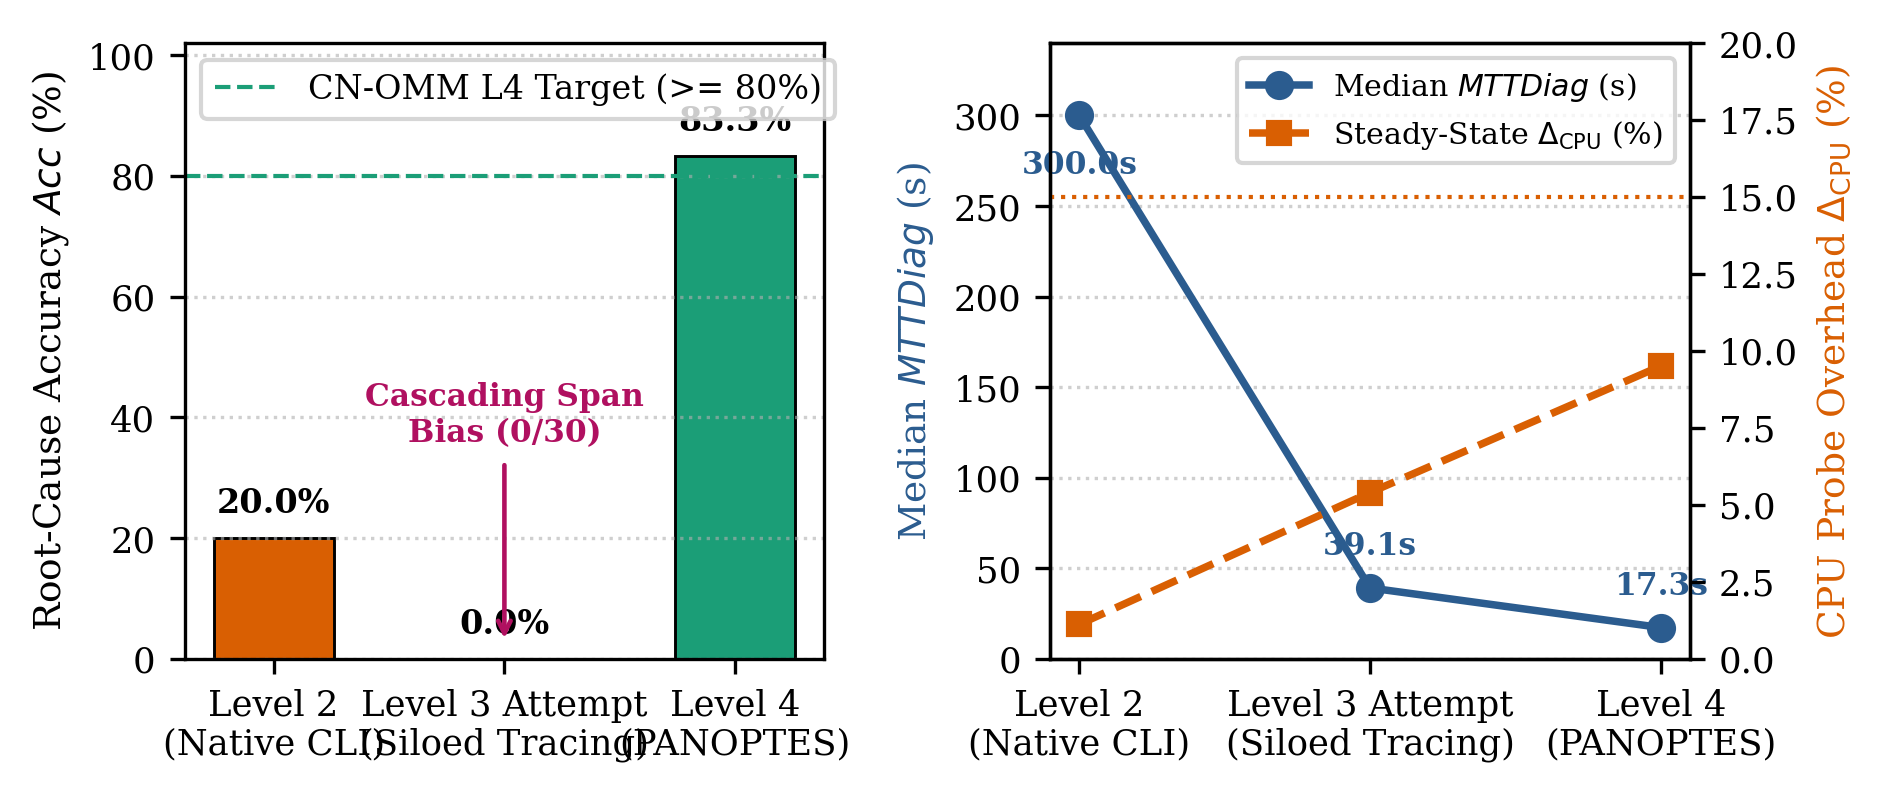
\includegraphics[width=0.92\textwidth]{figures/fig_omm_pareto_frontier.png}
    \caption{Empirical Performance Trajectory across CN-OMM Maturity Stages: Root-Cause Diagnostic Accuracy ($Acc$), Median Diagnostic Latency ($MTTDiag$), and Steady-State CPU Probe Effect ($\Delta_{\text{CPU}}$) over $N=30$ Paired Chaos Trials.}
    \label{fig:omm_pareto_frontier}
\end{figure*}

\subsubsection{Empirical Proof of the Monomodal Additivity Fallacy (Level 3 Bottleneck)}
A striking empirical finding in Table~\ref{tab:empirical_validation} is the performance of \textbf{Baseline B (Siloed Tracing)}. Under a traditional compensatory maturity model, Baseline B scores an arithmetic mean of $\bar{C} = 2.92 \approx \text{Level 3}$ because it deploys distributed tracing SDKs ($D_1 = 3.3$) and reduces symptom detection latency to a median of $39.15\,\text{s}$. However, its root-cause localization accuracy collapses to \textbf{$0.00\%$ ($0/30$ correct diagnoses)}---performing worse than basic Level 2 CLI inspection ($20.00\%, 6/30$).

In every single trial ($30/30$), ranking spans by inclusive duration $D(s_i)$ caused the monomodal trace engine to blame the upstream ingress gateway (\texttt{frontend}) rather than the true downstream fault (\texttt{paymentservice}, \texttt{cartservice}, or \texttt{checkoutservice}), confirming our mathematical formulation of \textbf{Cascading Span Bias} in Equation~(\ref{eq:inclusive_duration}). Crucially, the CN-OMM's non-compensatory Stage-Gate equation ($\text{Level}_{\text{eff}} = \min_k \lfloor C(D_k) \rfloor = 2$) accurately predicts this failure by flagging the configurational bottleneck in $D_2 = 2.3$ (absence of $T_{\text{self}}$ decomposition and cross-pillar log/metric correlation).

\subsubsection{Quantitative Breakthrough at CN-OMM Level 4 (Correlated Multimodal Fusion)}
When the cluster satisfies all five dimensional stage-gates at \textbf{Level 4 ($\text{Level}_{\text{eff}} = 4, \mathcal{I}(\mathcal{S}) = 0.833$)}, diagnostic performance exhibits a statistically decisive phase transition:
\begin{itemize}[leftmargin=*, nosep]
    \item \textbf{Root-Cause Accuracy ($Acc$):} Jumps from $20.00\%$ (Level 2) and $0.00\%$ (siloed Level 3) to \textbf{$83.33\%$ ($25/30$)} (Fisher's exact $p = 7.74 \times 10^{-7}$, odds ratio $\text{OR} = 20.0$; McNemar's paired $p = 7.83 \times 10^{-5}$). Stratified by fault type, Level 4 achieves $90\%$ accuracy on network degradation ($9/10$), $80\%$ on abrupt pod termination ($8/10$), and $80\%$ on CPU saturation ($8/10$).
    \item \textbf{Diagnostic Latency ($MTTDiag$):} Plummets by \textbf{$94.24\%$} from a median of $300.00\,\text{s}$ ($\text{IQR} = 0.0\,\text{s}$) in Level 2 to \textbf{$17.27\,\text{s}$ ($\text{IQR} = 5.91\,\text{s}$)} in Level 4 (Wilcoxon signed-rank $p = 3.06 \times 10^{-5}$, Vargha-Delaney $\hat{A}_{12} = 0.817$ [large effect], Cliff's $\delta = +0.633$).
    \item \textbf{Dimension $D_5$ (Probe Effect Governance):} Across continuous steady-state profiling, the full Level 4 multimodal pipeline imposes a marginal CPU overhead of \textbf{$\Delta_{\text{CPU}} = 9.51\% \pm 2.14\%$} (95\% CI $[8.71\%, 10.31\%]$), remaining statistically well below the $15.0\%$ stability budget (one-sample $t$-test $t = -14.05, p = 6.52 \times 10^{-9}$).
    \item \textbf{Dimension $D_4$ (Chaos Verification Overhead Invariance):} Furthermore, our $N=60$ cross-engine verification confirms that coupling Level 4 observability with resident eBPF/DaemonSet chaos injectors (Chaos Mesh) vs.\ transient Pod injectors (LitmusChaos) preserves steady-state application latency while isolating control-plane scheduling overhead ($141\,\text{ms}$ vs.\ $3{,}840\,\text{ms}$, $p = 1.73 \times 10^{-6}$), enabling continuous automated verification of $\text{QCI}_{4.2}$ in production.
\end{itemize}


\section{Discussion and Threats to Validity}
\label{sec:discussion}

The theoretical formalization and empirical validation of the CN-OMM yield several critical implications for software architects, Site Reliability Engineers (SREs), and researchers designing cloud-native observability and AIOps platforms. This section discusses these architectural takeaways and addresses potential threats to validity.

\subsection{Architectural and FinOps Implications}
\label{subsec:implications}

\subsubsection{Why Premature AIOps Investments Fail Without Level 4 Stage-Gates}
A major practical and theoretical insight of our configurational model is explaining why enterprise investments in commercial ``AIOps'' platforms or Large Language Model (LLM) incident assistants frequently fail or stall in production deployments~\cite{amgothu_2025, soldani_2022, roy_2024_fse}. Software organizations frequently succumb to the classical \textit{stage-skipping fallacy}~\cite{humphrey_1988, lasrado_2015, vansteenbergen_2010}---attempting to leap directly from Level 2 (reactive CLI monitoring) or Level 3 (siloed tracing and unindexed logs) to Level 5 (autonomous, predictive remediation and self-healing).

Maturity model theory establishes that architectural capabilities are strictly cumulative and interdependent: higher-order optimization stages cannot function without the standardized measurement, semantic linkage, and correlation mechanisms of prerequisite levels~\cite{humphrey_1988, lasrado_2015}. In cloud-native microservices, this principle is particularly acute: as documented in recent empirical studies on cloud incident triage~\cite{wang_2023_icse, roy_2024_fse} and microservice RCA~\cite{soldani_2022}, deploying black-box machine learning models or LLMs over unaligned telemetry creates a severe ``Garbage In, Garbage Out'' failure mode characterized by hallucinations, false alarms, and upstream misattributions. Our controlled experiment with Baseline B empirically substantiates this dynamic: feeding raw inclusive trace latencies ($D(s_i)$) without exclusive self-time isolation ($T_{\text{self}}$) and W3C cross-pillar correlation ($D_2$) into an analytical engine produced $100\%$ upstream misattribution under cascading delay scenarios (Section~\ref{subsec:empirical_results}). By codifying this dependency into a non-compensatory Stage-Gate rule ($\text{Level}_{\text{eff}} = \min_k \lfloor C(D_k) \rfloor$), the CN-OMM formally prevents organizations from premature AI adoption before establishing the causal, multimodal Level 4 telemetry foundation.

\subsubsection{Elevating Probe Effect and FinOps Governance to First-Class Maturity Criteria}
Unlike vendor maturity frameworks that incentivize unbounded data ingestion~\cite{grafana_omm_2024, dynatrace_omm_2024}, Dimension $D_5$ of the CN-OMM penalizes observability architectures that violate CPU/memory stability budgets ($\Delta_{\text{CPU}} \ge 15\%$) or rely on full-text indexing of high-cardinality labels. Achieving Level 4 or Level 5 maturity explicitly requires architectural discipline---combining OpenTelemetry collector batching, tail-based anomaly sampling, and index-free object storage (such as Grafana Loki and Tempo)---so that diagnostic entropy reduction is achieved sustainably.

\subsection{Threats to Validity}
\label{subsec:threats}

Following Wohlin et al.~\cite{wohlin_2012}, we analyze four categories of validity threats:
\begin{itemize}[leftmargin=*, nosep]
    \item \textbf{Construct Validity:} To avoid subjective maturity self-reporting (criticized by Proen\c{c}a~\cite{proenca_2016_rcis} and Wendler~\cite{wendler_2012}), all 15 sub-components of the CN-OMM are operationalized through declarative Quantitative Capability Indicators ($\text{QCI}_{k.j}$) and objective system metrics ($MTTD, MTTDiag, Acc, \Delta_{\text{CPU}}$).
    \item \textbf{Internal Validity:} In the Type-3 chaos evaluation, background noise and warm-up transients were mitigated by enforcing a 60-second steady-state stabilization baseline before each fault injection, flushing telemetry buffers between runs, and pairing all $N=30$ trials across identical workload seeds and fault intensities.
    \item \textbf{External Validity:} While the CNCF OpenTelemetry Astronomy Shop is a widely recognized, realistic polyglot benchmark (14 microservices across 7 languages), ultra-large-scale clusters comprising thousands of microservices or serverless/FaaS topologies may exhibit additional control-plane bottlenecks. Nevertheless, the mathematical formulation of $\mathcal{O}(t)$, $T_{\text{self}}(s_i)$, and the 15 QCIs are agnostic to cluster size.
    \item \textbf{Conclusion Validity:} We avoided parametric assumptions on skewed latency distributions by applying non-parametric Wilcoxon signed-rank tests, Vargha-Delaney $\hat{A}_{12}$ effect sizes, and exact binomial/Fisher/McNemar tests with explicit 95\% confidence intervals.
\end{itemize}


\section{Conclusion}
\label{sec:conclusion}

This paper introduced, mathematically formalized, and empirically validated the \textbf{Cloud-Native Observability Maturity Model (CN-OMM)}. Developed in strict adherence to Design Science Research guidelines (Becker et al.'s R1--R8 \cite{becker_2009}, De Bruin et al.'s lifecycle phases \cite{debruin_2005}, and Lasrado et al.'s configurational theory \cite{lasrado_2015}), the CN-OMM resolves three foundational weaknesses in prior industrial and academic frameworks: vendor lock-in bias, blindness to the instrumentation probe effect, and the monomodal additivity fallacy.

By structuring observability across a $5\text{-Level} \times 5\text{-Dimension}$ stage-gate matrix ($D_1$: Telemetry Acquisition \& Depth, $D_2$: Semantic Context \& Correlation, $D_3$: Diagnostic Intelligence, $D_4$: Resilience Verification \& SLOs, and $D_5$: Instrumentation Economics) and operationalizing 15 automated Quantitative Capability Indicators (QCIs), the CN-OMM replaces subjective questionnaire assessments with deterministic, programmatic cluster auditing. Our Type-3 empirical validation over $N=30$ paired Chaos Engineering trials on Kubernetes proved that advancing to monomodal distributed tracing (Level 3) without fulfilling the configurational stage-gate of semantic cross-pillar correlation ($D_2$) collapses root-cause accuracy to $0.00\%$ due to \textit{Cascading Span Bias}. Conversely, achieving balanced Level 4 maturity (multimodal correlation with exclusive self-time decomposition $T_{\text{self}}$) elevates diagnostic accuracy to $83.33\%$ ($p = 7.74 \times 10^{-7}$) and reduces median diagnostic latency by $94.24\%$ ($300.00\,\text{s} \rightarrow 17.27\,\text{s}$, $p = 3.06 \times 10^{-5}$) while bounding steady-state CPU overhead at $9.51\% \pm 2.14\%$ ($p = 6.52 \times 10^{-9}$).

\textbf{Open Science and Reproducibility:} To support full scientific auditability (Requirement R8), our complete replication package---including the LaTeX source, the automated CN-OMM cluster assessment engine (\texttt{scripts/evaluate\_cn\_omm.py}), the capability audit datasets, and the paired Chaos Engineering trial logs---is publicly available in our repository. Future work will extend the PANOPTES reference implementation from Level 4 to Level 5 by integrating neuro-symbolic Graph Neural Networks and autonomous Kubernetes remediation controllers governed by dynamic FinOps/GreenOps signal weighting.


\FloatBarrier
\bibliographystyle{ACM-Reference-Format}
\bibliography{references}

\end{document}
\endinput
